\title{Khakhalin. Graph analysis of collision detection networks}

%\documentclass[twocolumn]{article}
\documentclass{article}

\usepackage[utf8]{inputenc}
\usepackage[top=0.85in,left=1.5in,right=1.5in,footskip=0.75in]{geometry} % For one-column version
%\usepackage[top=0.85in,left=1in,right=1.0in,footskip=0.75in]{geometry} % For two-column version
% marginparwidth=2in

\usepackage{helvet} % Set font to Arial-like
\renewcommand{\familydefault}{\sfdefault} % Force this font

\usepackage[round, sort, numbers, authoryear]{natbib} % Reference manager, round citations
% \usepackage[super]{natbib} % Nature-style citations
% \setcitestyle{citesep={,}} % For nature-style, comma instead of ;

%\usepackage[switch,pagewise]{lineno} % Numbered lines for two columns
\usepackage[pagewise]{lineno} % Numbered lines for one column

%\usepackage{adjustbox} % To change margins around a table. Doesn't work?
\usepackage{tabularx} % To set table column width, if needed
\usepackage{rotating} % To write text sidewise
\usepackage{xcolor}
\renewcommand{\linenumberfont}{\normalfont\bfseries\small\color{lightgray}}
\definecolor{linkcolor}{rgb}{0.2,0.6,0.7} % Neuron-style link color
\usepackage[colorlinks=true,citecolor=linkcolor,urlcolor=blue]{hyperref}%
%\usepackage{url}

% improves typesetting in LaTeX
\usepackage{microtype}
\DisableLigatures[f]{encoding = *, family = * }

% this package is supposed to give access to upright mu symbol via \micro
%\usepackage{siunitx} % didn't work for some reason
\usepackage{amsmath} % to enable \text tag
\usepackage{amssymb} % to enable \leqslant

% text layout
\raggedright
%\textwidth 6in 
%\textheight 9in
\setlength{\parindent}{0em}
\setlength{\parskip}{1em}

% adjust caption style
\usepackage[aboveskip=5mm,labelfont=bf,labelsep=period,singlelinecheck=off]{caption}

% this is required to include graphics
\usepackage{graphicx}

% Multicolumns
\setlength{\columnsep}{1cm}

% Headers and footers
\usepackage{fancyhdr}
\pagestyle{fancy}
\rhead{Khakhalin AS. Graph analysis of collision detection networks. (EARLY DRAFT) Page \thepage}
\cfoot{} % To kill footer page numbers

\begin{document} % --------------------- Document start ----------------

%TC:ignore 
% The comment above is for textcount to ignore this text.
% It will ignore everything until the endignore pair, and so on.
% We need to get down to 4500 words in the main text.

\linenumbers % Comment to suppress line numbers

% title goes here:
%\twocolumn[
\begin{flushleft}
{\Large
\textbf\newline{Graph analysis of collision detection networks in the tectum, and its replication in a simple computational model (EARLY DRAFT)}
}
\newline
% authors go here:
\\
Arseny S. Khakhalin\textsuperscript{1,*}
\\
\bigskip
{1} Biology Program, Bard College, Annandale-on-Hudson, NY. 

* Correspondence: khakhalin@bard.edu

\section*{Abstract}
Looming is one of the most salient visual stimuli an animal may encounter, yet mechanisms of looming detection in vertebrates are poorly understood. For many animals, key computations involved in looming detection and collision avoidance seem to be performed by distributed networks, making it hard to tease out the underlying mechanisms. In this study, we contrast a computational developmental model of the optic tectum with the analysis of directed connectivity graphs, reconstructed from high-speed calcium imaging recording in \textit{Xenopus} tadpoles. We report a difference in degree distributions and modularity of tectal networks reconstructed from younger and older tadpoles. We also describe that looming-selective cells in the tectum tended to receive more inputs, and had higher Katz centrality than non-selective cells. We compare these results to predictions from a model governed by spike-time-dependent plasticity, homeostatic intrinsic plasticity, synaptic competition, and driven by structured visual inputs. We show that under general conditions, the model network developed robust looming selectivity, and replicated some network changes observed in imaging experiments, including changes in modularity and degree distribution. Other changes predicted by the model (hierarchy, efficiency, and spatial distribution of selective cells) were however not observed in imaging experiments. Finally, by comparing several reduced models, we predict which developmental rules could be most critical for the development of looming selectivity in the brain.
%TC:ignore 
\bigskip

\end{flushleft} % Only relevant for two-column documents, but doesn't hurt
%] % End of one-column region

\section*{Introduction}

Few sensory stimuli are as conspicuous and ill boding as visual looming. A retinal projection that is small, but quickly grows in size, may promise either a painful collision, or a meeting with a hungry predator, and so it inherently calls for an action, such as an avoidance maneuver, freezing, defensive posturing, or a blink. Moreover, looming detection has to be fast to be meaningful. Not surprisingly, it is described in virtually every type of animals that uses vision, from insects to primates \citep{Pereira2016}.

In different animals, looming detection seems to rely on a variety of networks and solutions [Frost Sun 2004], including dimming detectors in the retina \citep{ishikane2005,munch2009}, opponent motion detection \citep{klapoetke2017looming}, and competitive spike-frequency adaptation \citep{peron2009adaptation,fotowat2011multiplexing}. Even within a single clade of anuran amphibians (frogs), animals seem to employ several competing looming detection mechanisms, such as non-linear detection of retinal oscillations \citep{baranauskas2012}, and rebound of recurrent activity \citep{jang2016}. Moreover, it seems that at least some of these competing mechanisms may lead to different subtypes of avoidance responses, as it was described in insects \citep{card2008tradeoffs,chan2013avoidance}, fish \citep{burgess2007twoescapes,portugues2009behaviors,budick2000repertoire,temizer2015pathway,bhattacharyya2017assessment}, and tadpoles \citep{khakhalin2014}.

While this co-existence of multiple alternative solutions for looming detection may seem overwhelming, it actually matches the recent insight from the field of machine learning. Simple, crude ways of detecting important features of sensory stimuli are critical for training more sophisticated and efficient networks, that are then used for more nuanced analysis of the sensory world at later stages of development \citep{marblestone2016deeplearning}. In case of looming stimuli in tadpoles, early in development, when collision detection is weak \citep{dong2009}, animals may use “hardwired” dimming receptors in the retina to detect collisions, but also to “bootstrap” more sophisticated motion-dependent networks in the tectum. Later, these motion-dependent networks can serve as a first line of defense, identifying early phases of looming, and providing information to motor neurons in the hindbrain to perform course correction \citep{khakhalin2014,bhattacharyya2017assessment}, yet dimming detectors could remain as a backup, and mediate a more urgent and less coordinated response. Moreover, every time collision avoidance is not performed perfectly, these sensorimotor networks can be further refined, relying on inputs from the lateral line and mechanosensory detectors in the skin \citep{felch2016}.

Traditionally, the golden standard for describing a mechanism of a behavior was to demonstrate that activation of a certain structure is both sufficient and required for this behavior \citep{krakauer2017reductionist}. This reductionist approach works well in some systems, such acoustic startle detectors \citep{korn2005mauthner}, or central pattern generators in the spinal cord \citep{roberts2010hatchling}, that are compact and isolated enough. Yet most systems in the brain act as complex, interconnected, distributed dynamical systems, which makes it hard to represent them as a sum of “parts”, with distinct functions ascribed to each of these parts \citep{gao2015simplicity}. It is possible to study these complex systems statistically, identifying properties that hold “on average”, and differ in functional and dysfunctional networks, but a statistical approach typically does not grant true insight into the “meaning” of these properties \citep{bassett2018models}. For example, knowing that a disordered brain does not adhere to the same network statistics as a normal brain would not necessarily tell us how to “fix” it, even if we had a method to rewire individual neurons in a targeted fashion.

A more promising approach is to study the origin of functional structures in the brain. Most neural networks are not truly hardwired, but dynamically evolve from a set of developmental rules [xxxnon-Pietri ref], similar to how it happens for Turing patterns or fractals \citep{lefevre2010reaction,bullmore2012economy}, while also relying on streams of structured sensory information coming from the external world \citep{gao2015simplicity}. This insight is encouraging, as these developmental rules are followed by individual cells and their compartments, such as dendrites and synapses, which implies that while the ultimate product of these rules is exceedingly complex, the rules themselves have to be relatively simple \citep{bassett2018models}. Together, it may mean that our best chance to truly “understand” the brain lies in identifying the space of rules that lead to the development of functional networks \citep{linderman2017constrain}. This general approach already proved to be fruitful, as several complex network phenomena, including high-order receptive fields \citep{bashivan2018neural}, grid cells \citep{banino2018grid}, and decision circuits \citep{haesemeyer2018convergent}, were shown to evolve spontaneously in systems governed by intuitive developmental rules. 

In this paper, we look at connectomic correlates of looming selectivity in the developing optic tectum of \textit{Xenopus} tadpoles. Tadpole tectum is a model uniquely suitable for studies of sensory integration, as its neurons are excessively plastic \citep{pratt2007intrinsic}[Busch], strongly connected to each other \citep{james2015}[refs], and develop reliable looming selectivity within about a week, as tadpoles mature from developmental stage 46 to stage 49 \citep{dong2009,khakhalin2014}. The refinement of tectal connectivity is dominated by spike-time-dependent plasticity \citep{zhang1998stdp,mu2006stdp}, which is known to favor development of synfire chains \citep{fiete2010chains,zheng2014synfire}: groups of neurons linked with sequential connections that selectively respond to certain patterns of temporal activation \citep{clopath2010stdpcoding}. As  tectal neurons spike relatively slowly, with broad spikes and long refractory periods \citep{ciarleglio2015,jang2016}, these synfire chains are expected to have delays of about 10 ms from one neuron to another, compared to $\sim$2 ms in the mammalian cortex [ref]. This slower signal propagation brings intratectal connections to the threshold of direct detectability by fast Ca imaging techniques that operate at rates of ~100 frames/s, allowing observations of not just co-firing of neurons within each ensemble or clique \citep{reimann2017,avitan2017spontaneous}, but propagation of signal through these ensembles.

Here we use high-speed Ca imaging data to infer connectivity of small sub-networks within the tectum, describe connectivity patterns in younger and older tadpoles, and compare them to predictions from a simple developmental simulation. We hypothesized that by comparing statistical properties of networks generated by a family of models to networks reconstructed in imaging experiments we would be able to reverse-engineer developmental rules that govern development of looming-sensitive networks in the tectum. We show that our model predicted some, but not all aspects of topology and functionality in looming-sensitive networks, and that both matches and contradictions between the model and the experiment are not clear enough to draw simple conclusions. Nevertheless, we report several new findings, including some very surprising negative results, and as a proof of concept, demonstrate looming detectors can emerge in developing networks through a simple interplay of structured inputs and plasticity.

\section*{Results}

For all mathematical methods, we provide their names and their interpretation in the main text, but leave definitions and details for the “Methods” section. For statistical analyses, we report p-values without correction, and interpret them according to Fisher, and not Neyman-Pearson philosophy \citep{greenland2016}. This approach is preferable for this study, as many of our analyses are not independent, but still ask different questions, and rely on different null model hypotheses. At the interpretation step, we pay more attention to hypotheses supported by several alternative analyses.

We performed Ca imaging in 14 stage 45-46 tadpoles, and 16 stage 48-49 tadpoles, recording responses from 128$\pm$40 tectal cells (between 84 and 229; here and below “$\pm$” after the mean denotes standard deviation). Unless stated otherwise, sample sizes $n=$ 14 and 16 animals for stage 46 and 49 tadpoles respectively apply to all analyses between younger and older animals reported in this study. To each tadpole, we presented a sequence of three different stimuli, always in the same order: a looming stimulus, followed by a full-field flash, followed by a spatially “scrambled” looming stimulus (Fig 1A). Scrambled stimuli were identical to looming, except that the visual field was split into a 7x7 grid of square tiles, and these tiles were randomly rearranged in space. In total we presented 60$\pm$11 stimuli to every animal, which means that a stimulus of every type was presented 20$\pm$4 times. High speed calcium imaging signals \citep{xu2011,truszkowski2017} were recorded from one layer of “deep” principal tectal neurons in the tectum (Fig 1B,C); from these videos we then extracted fluorescence traces (Fig 1D,E), and inferred average spiking of each neuron within every frame (Fig 1F,G).

\begin{figure*}
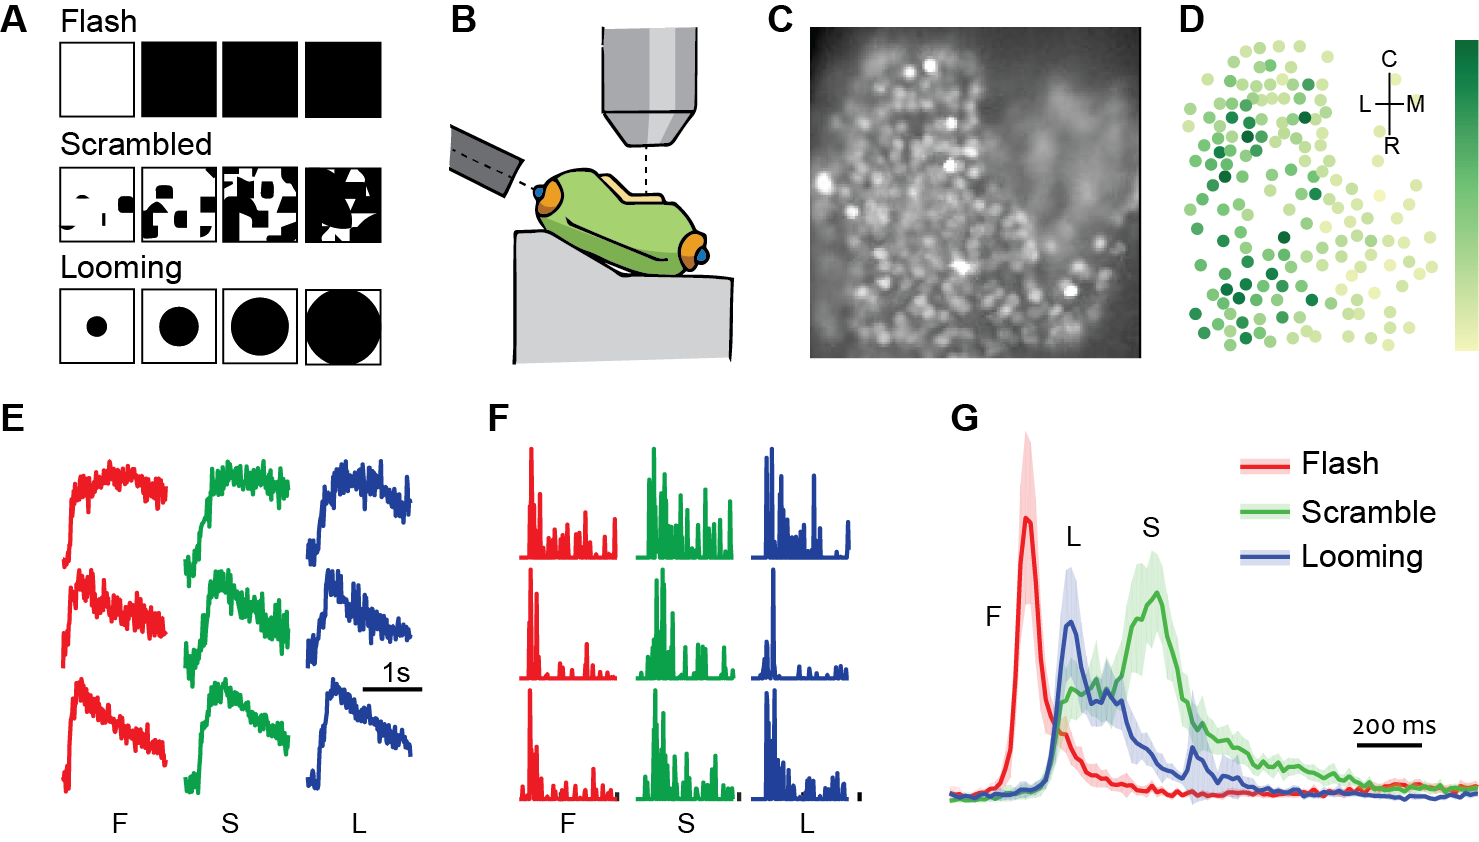
\includegraphics[width=\linewidth]{fig1.png}
\caption{
Overview of experimental design. \textbf{A}. Four representative frames from visual stimuli of each type. \textbf{B}. Schematic of the preparation. \textbf{C}. View of the optic tectum during the calcium imaging recording. \textbf{D}. Matching regions of interest and average responses in each cell. \textbf{E}. Typical fluorescence responses to flash (F), scramble (S) and looming (L) stimuli from three cells in the tectum. \textbf{F}. Spiking estimations for these fluorescence traces. \textbf{G}. Average full-brain responses to stimuli of every type, wich 95\% confidence interval band, for one representative experiment. }
\end{figure*}

\subsection*{Responses and stimulus selectivity}

Similar to previously published electrophysiology experiments \citep{khakhalin2014}, responses to flashes were fast, with a sharp peak and mild recurrent activation after the peak, while responses to looming stimuli were slower, and followed by strong recurrent activation (Fig 2A). Responses to both looming and scrambled stimuli were highly variable from one animal to another; for scrambled stimuli this can be easily explained, as frame tiles were rearranged differently in different experiments, increasing response variability. For looming stimuli however, this may indicate either an inherent variability of network configuration from animal to animal, or different levels of recurrent inhibition across preparations. We did not quantify differences in response shapes, and proceeded with the analysis of response amplitudes.

The total output of observed tectal networks tended to be higher in response to looming stimuli than to flashes (on average, 39$\pm$29\% higher for younger; 25$\pm$25\% higher for older tadpoles; $p_{t1}=$ 2e-4 and 1e-3 respectively; Fig. 2B). There was no change in this preference in development ($p_t$=0.15). Responses to looming and scrambled stimuli did not differ (average differences of $-$0.03$\pm$0.15 and $-$0.01$\pm$0.20; $p_{t1}=$ 0.45 and 0.78 for younger and older animals respectively), and there was no different in development ($p_t=$ 0.80). This supports our prior observations that in tadpoles, the total tectal response depends mostly on the dynamics of visual stimuli, rather than on their geometry \citep{khakhalin2014,jang2016}.

\begin{figure*}
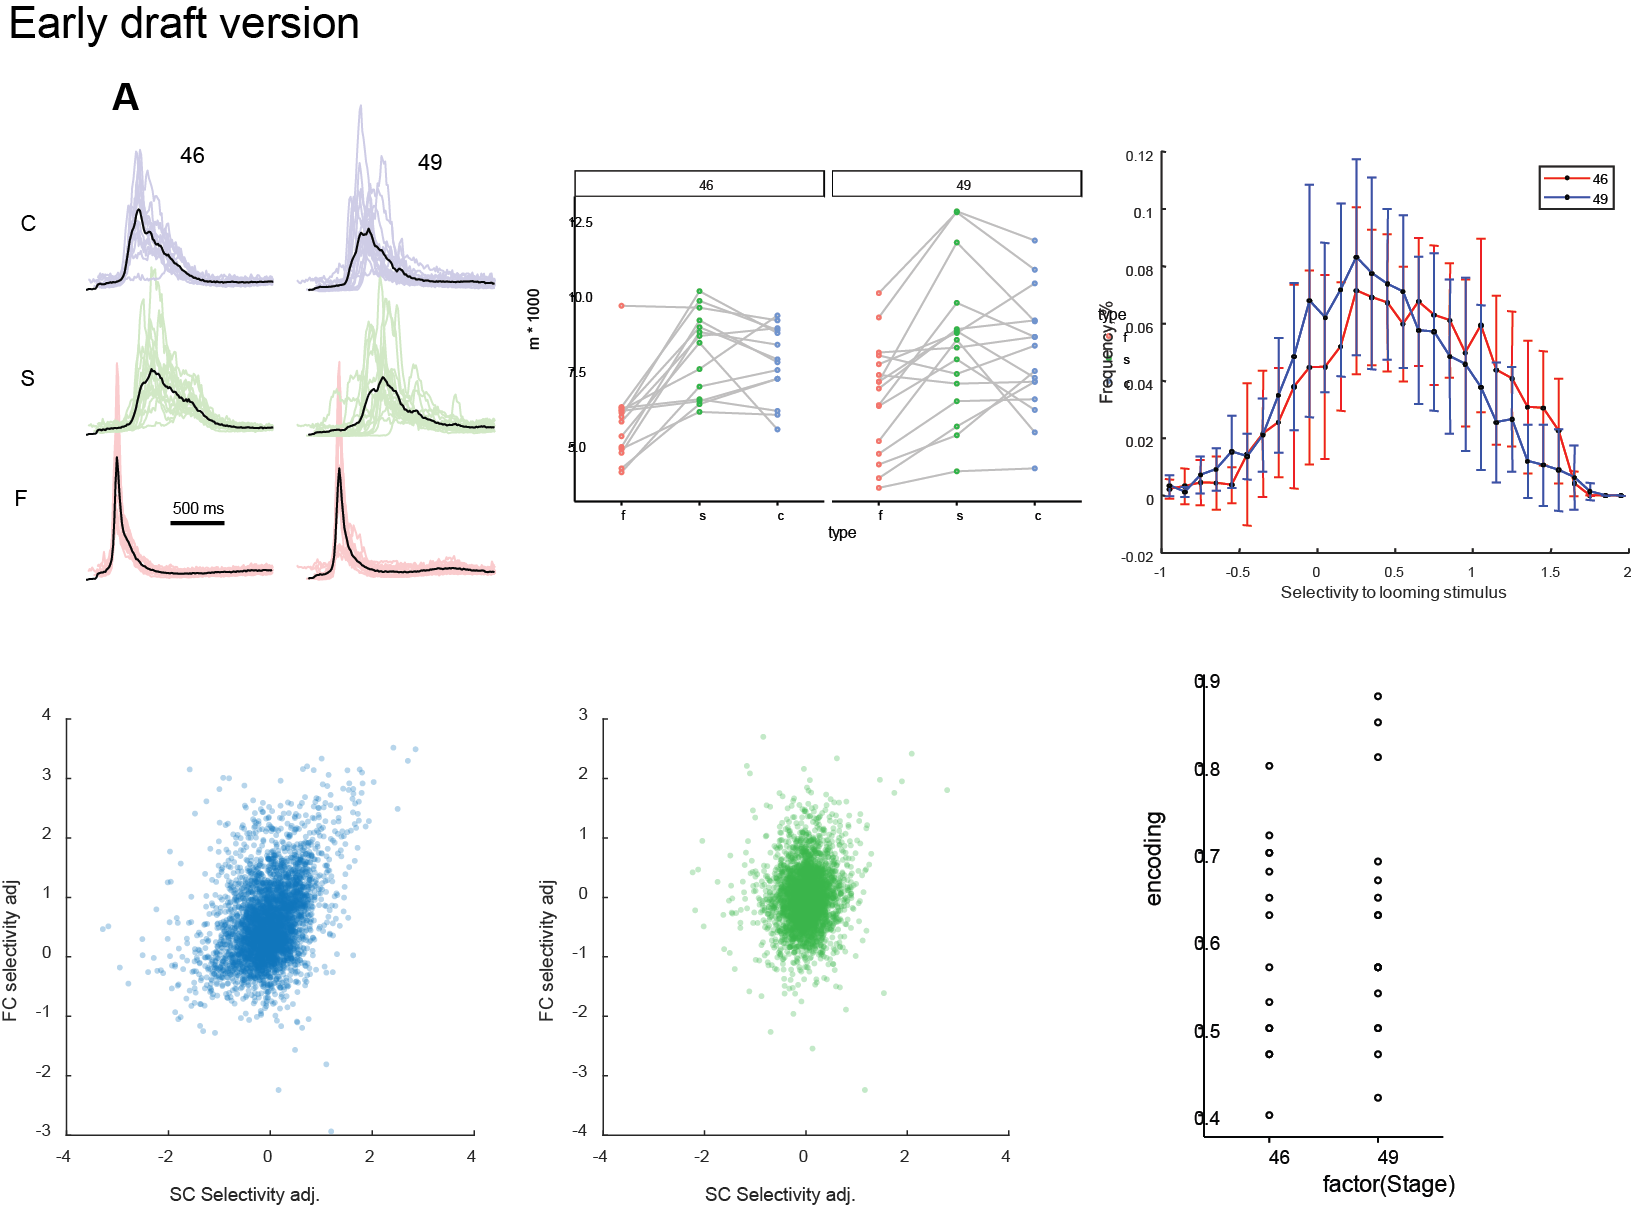
\includegraphics[width=\linewidth]{fig2.png}
\caption{
Selectivity analysis. \textbf{A}. \textbf{B}. \textbf{C}. \textbf{D}. \textbf{E}. \textbf{F}. }
\end{figure*}

To quantify selectivity of individual tectal cells, we calculated Cohen’s $d$ effect size for each cell (the difference in means, divided by the pooled standard deviation), comparing cumulative responses to different stimuli. We considered two measures of selectivity: that for "looming over flash" (a type of selectivity that may rely on both stimulus dynamics and its spatial organization), and "looming over scrambled" (that can only rely on spatial organization of stimuli, as they had the same dynamics). On average, tectal cells were selective for looming stimuli (within-brain mean $d$ of 0.67$\pm$0.50 and 0.46$\pm$0.47 in younger and older tadpoles respectively), and there was no difference between stages ($p_t=$ 0.3). The share of cells that responded to looming stimuli stronger than to flashes also did not change in development (84$\pm$23\%, 77$\pm$21\%; $p_t=$ 0.4). There was however a developmental change in the distribution of cell selectivity values within each brain: while the variance did not change ($p_t=$ 0.3), there was a change in skew ($p_t=$ 0.02), which was positive in younger animals, but negative in older ones, reflecting a decrease in number of top-selective cells within each brain (Fig. 2I). A more intuitive way to quantify this difference is by looking at the gap between top-selective (90th percentile) and median selective cells, which went down in older animals (0.75$\pm$0.26 in younger, but 0.53$\pm$0.27 in older tadpoles; $p_t=$ 0.03). Overall, these results were quite unexpected: in collision avoidance tests stage 49 tadpoles perform better than stage 46 tadpoles \citep{dong2009}, and we expected them to develop a subset of looming-selective cells, as described in adult frogs \citep{nakagawa2010otneurons,baranauskas2012}, and other vertebrates \citep{wang1992pigeon,wu2005pigeon,liu2011cat}. Yet in our experiments selectivity for looming stimuli did not change, and a subpopulation of strongly selective cells not only did not emerge in older animals, but became less prominent.

We then considered the second, more computationally demanding definition of selectivity: a preference for spatially organized looming stimuli over scrambled stimuli. On average, tectal cells did not respond stronger to either of these stimuli (average selectivity of $-$0.07$\pm$0.33 in younger tadpoles, $-$0.04$\pm$0.49 in older ones), and the value of average selectivity did not change in development ($p_t=$ 0.9). The share of cells that responded to looming stronger than to scrambled was at a chance level for both developmental stages (46$\pm$31\%, 48$\pm$37\%, $p_t=$ 0.9), and there was no change in either within-brain variance of this selectivity ($p_t=$ 0.9), or the 90$-$50 percentile asymmetry of values ($p_t=$ 0.8).

The selectivity for scrambled stimuli over flashes correlated with selectivity for looming stimuli over flashes in both developmental groups: within-brain $r=$ 0.82$\pm$0.13, $p_{1t}=$3e-12 for younger animals, and 0.75$\pm$0.18, $p_{t1}=$ 3e-11 older ones (Fig 2D); no change in development ($p_t=$ 0.3). On the contrary, the preference for looming over flashes did not correlate with preference for looming over scrambled (Fig 2E; $r=$ 0.03$\pm$0.29, $p_{1t}=$ 0.7 for stage 46; 0.13$\pm$.30, $p_{1t}=$ 0.1 for stage 49). This further suggests that at least the majority of cells in the tectum responded to stimulus dynamics, rather than to its geometry.

Finally, as a most holistic way to quantify tectal network selectivity, we looked at the total power of tectal responses to predict stimulus identity \citep{avitan2016limitations}, known as "stimulus encoding" [XXX]. We ran a logistic regression on one half of the data, linking amplitudes of tectal cells responses in each trial to the type of stimulus used in this trial. Then we measured the quality of this linkage on the second half of recorded data (Fig. 2F). The quality of prediction was rather low: 59$\pm$12\% for younger, and 62$\pm$13\% for older tadpoles, with no change in development ($p_t=$ 0.6).

To assess cell-to-cell variability of responses, we performed exploratory factor analysis (principal component analysis, followed by promax rotation) of responses within each preparation. We restricted analysis to looming stimuli, as otherwise factor analysis detected cell-to-cell differences in selectivity, while we wanted to look at differences in dynamics within a single response type. The first and second principal components explained on average 19$\pm$7\% and 4$\pm$1\% of variance in younger tadpoles, and 24$\pm$14\% and 3$\pm$1\% in older tadpoles, and were largely different response timing (Fig. 3A). Early responding cells tended to group together in one part of the recorded field (Fig. 3B), and we were able to quantify the position of this early responding group of cells in each experiment, by maximizing the correlation between distances to the center of interest, and relative scores of the early response component in each cell. The fit was robust, with $p<$ 0.05 in every experiment (30/30), and average achieved correlation of $r=$ 0.59$\pm$0.23. To assess possible overfitting, we performed same analysis after reshuffling cell identities 5 times for each experiment, which yielded average $r$ values of only 0.13$\pm$0.06, and $p_r<$ 0.05 in 21\% of experiments. From this we concluded that spatial clustering of cells with early responses to looming stimuli was not an artifact of analysis, even though "optimization of correlations" exaggerated its effect. We interpreted spatial clustering of early-responding cell is a manifestation of a retinotopic map well known to exist in the tectum \citep{ruthazer2004map}, as this map reproduced a looming stimulus projected on the retina. Across cells, the latency of average response correlated with distance from the retinotopy center ($r=$ 0.35 $\pm$ 0.24; correlations individually significant in 25/30 experiments), despite our latency estimations being noisy, especially for low-amplitude cells. Curiously, while visual projections to the tectum are known to be actively remodeled in development \citep{sakaguchi1985refinement,ruthazer2004map,munz2014hebbian}, the quality of functional retinotopic map did not differ between younger and older tadpoles, at least judging from correlations between early component prominence and cell position, that did not change in development (Fig. 3E; $r=$ 0.63 $\pm$ 0.21 and 0.57 $\pm$ 0.25 respectively, $p_t= $0.5), similar to reports in Zebrafish \citep{avitan2016limitations}.

\begin{figure*}
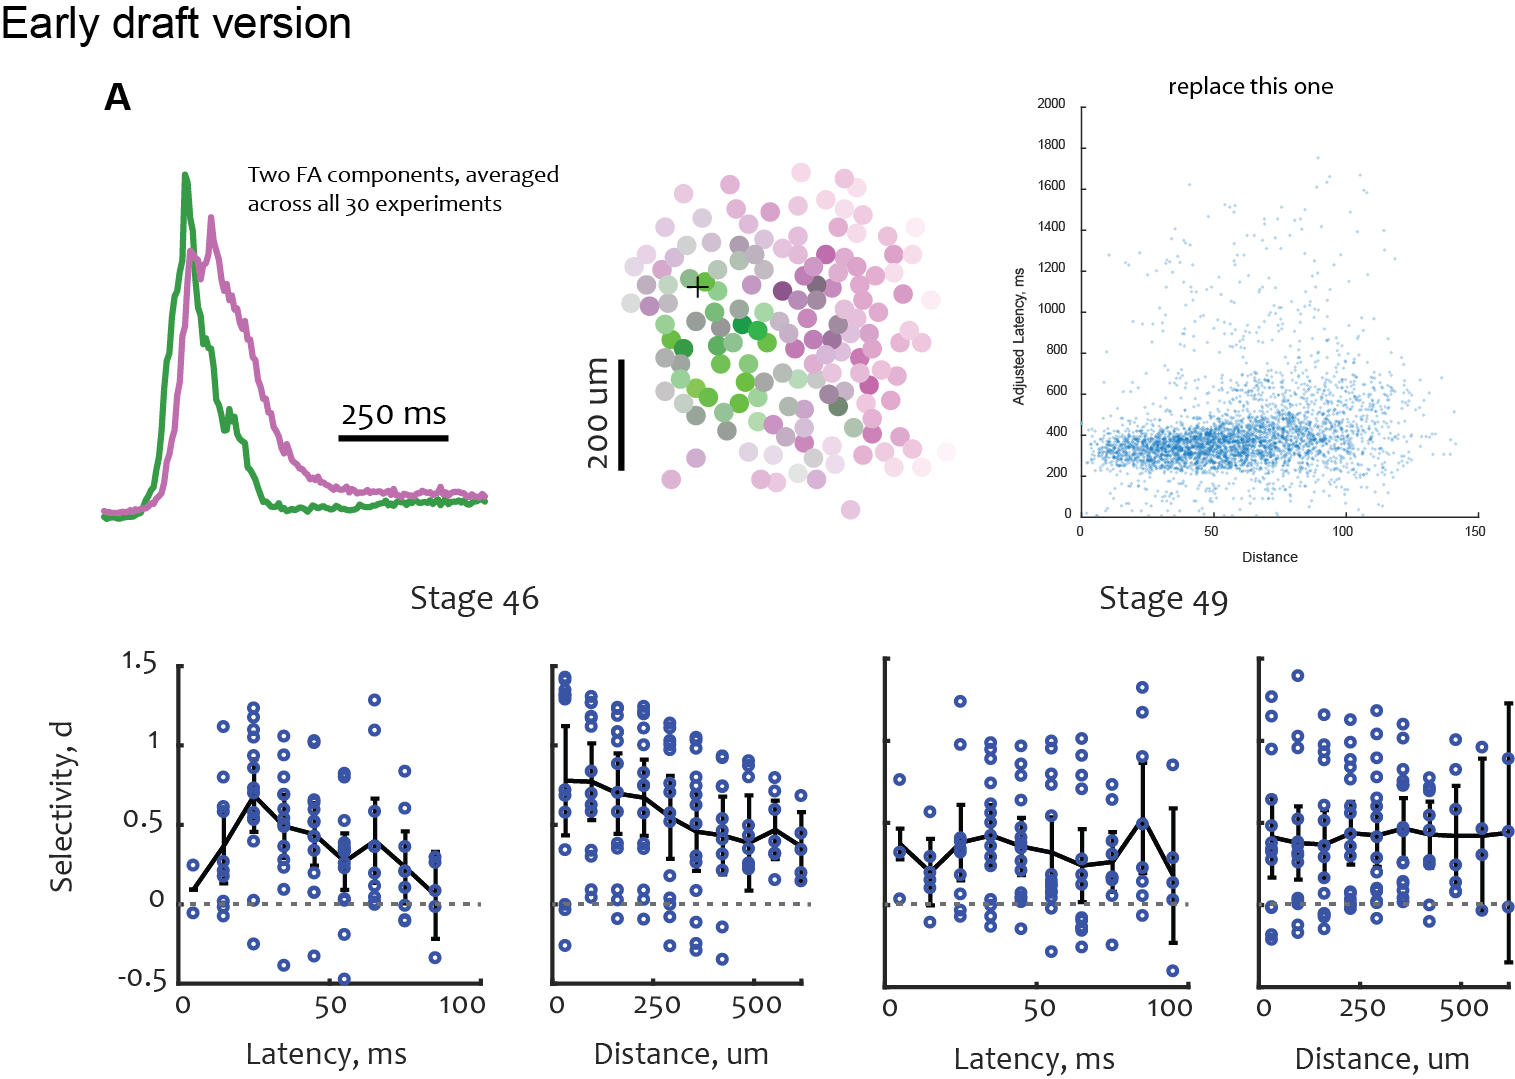
\includegraphics[width=\linewidth]{fig3.png}
\caption{
Spatial variability. \textbf{A}. \textbf{B}. \textbf{C}. \textbf{D}. \textbf{E}. \textbf{F}. }
\end{figure*}

Knowing where the looming stimulus responses originated within the tectum, we could then check whether looming-selective cells were more likely to be found in the center of the expanding activation area (as it would be expected if collision detection was retinotopic \citep{frost2004review} and based on feedback excitation \citep{jang2016}, or at the periphery, as predicted by the synfire model \citep{clopath2010stdpcoding,fiete2010chains}. We found that selectivity for looming stimuli over flash tended to decrease with distance from the estimated projection center (Fig. 3G) for both stage 45 (average $r=-$0.37$\pm$0.27; individual correlations $p_r<$0.05 in 12/14 experiments), and stage 49 tadpoles (average $r=-$0.09$\pm$0.35; $p_r<$0.05 in 12/16 experiments), indicating that looming-selective cells tended to be located in the center of the emerging spatial response. Similarly, at both developmental stages, selectivity decreased with response latency (stage 46: $p_r<$0.05 in 11/14 animals, average $r=-$0.29$\pm$0.11; stage 49: $p_r<$0.05 in 10/16 animals, average $r=-$0.16$\pm$0.21). Both correlations were weaker in older tadpoles ($p_t=$ 0.02 for distance-selectivity, $p_t=$ 0.03 for latency-selectivity), indicating a more uniform distribution of looming-selective cells within the network.

% Note that here selectivity is based on total responses across a whole second, and so much of this spiking happens really late. As a result, cells that spike early are also sensitive. But it's not clear whether it's actually because they are selective (get more relevant activation), or just can be activated for longer (because they start earlier), or because they receive some later recurrent activation (which would be real, but not relevant for collision avoidance)

% Similarly, if this thing is not observed in modeling experiments, it may be due to the absence of delayed recurrent excitation, which we didn't introduce into this model, but which is also not relevant for collision avoidance, as it just happens too late.

\subsection*{Variability and ensembles}

We then assessed the \textbf{trial-to trial variability} of tectal responses, to see whether it changed in development, as it was reported for variability of spontaneous activity \citep{xu2011}. We performed principal component analysis of response waveforms, and looked at the total number of components that was needed to describe 80\% of variability in the data \citep{avitan2017spontaneous}. We found that this number was similar in stage 46 and 49 tadpoles, with a minor increase in response richness in older animals (insignificant for each stimulus alone, but consistent across stimuli): 51$\pm$14 and 65$\pm$28, $p_t$=0.1 for responses to looming stimuli; 49$\pm$12 and 62$\pm$32, $p_t$=0.2 for flashes; 51$\pm$14 and 64$\pm$26, $p_t$=0.1 for scrambled stimuli.

To describe network activation variability, we used spectral clustering technique to find \textbf{ensembles} of tectal cells that were either active together, or silent together on a trial-by-trial basis \citep{thompson2016ensembles}. Unlike for recordings of spontaneous activity, we could not easily aggregate activity states into clusters \citep{avitan2017spontaneous}, as activation in our networks was driven by shared sensory inputs. Instead, we subtracted normalized average responses of each cell from its responses in individual trials, and calculated pairwise correlations on the remaining “anomalies” of trial-by-trial activation (see “Methods”). We turned these pairwise correlations into pairwise distances in a multidimensional space, ran a series of spectral clustering partitions \citep{ng2002spectral}, and of all possible partitions, picked the one that maximized spectral modularity \citep{newman2006modularity,gomez2009community}. We found that the number of ensembles did not differ between younger and older tadpoles (10$\pm$5 in stage 45, 11$\pm$11 in stage 49; $p_t$=0.9; Fig. 3X), but in older tadpoles ensembles were less isolated from each other, producing lower values of network modularity (0.14$\pm$0.05 to 0.09$\pm$0.06, $p_t$=0.03; Fig). This implies stronger coordination between ensembles in older tadpoles. Tectal ensembles also tended to be spatially localized (Fig. 3X): cells that shared an ensemble were on average closer to each other than to cells from different ensembles, for both younger (29$\pm$9\% closer) and older animals (25$\pm$10\% closer; no difference in development $p_t$=0.3).

\subsection*{Network reconstruction}

The high speed of video acquisition used in this study (83 frames/s) allowed us to look not just at instantaneous correlations between activity levels of individual neurons, but at the propagation of signals through the network. In \textit{Xenopus} preparations, it takes about 5 ms for a presynaptic action potential to evoke neurotransmitter release in a typical tectal synapse \citep{khakhalin2012}, and about 10 ms for a typical synaptic current to depolarize postsynaptic neuron above the spiking threshold \citep{ciarleglio2015}[Busch 2018], which makes the frame-to-frame delay in our video recordings (12 ms) ideally posed to infer neuronal connections from activity.

To reconstruct network connectivity, we calculated transfer entropy \citep{gourevitch2007te,stetter2012te}. Intuitively, for each pair of neurons $i$ and $j$ we quantified the amount of additional information that past activity of neuron $i$ can provide to predict current activity of neuron $j$. This is similar to calculating a cross-correlation between the activity of neurons $i$ and $j$ in frames $t$ and $t+1$ respectively, but unlike for a correlation, transfer entropy does not make assumptions about the function that links activities of neurons $i$ and $j$. It means that in a general case, TE has a higher power to detect causal links in the network \citep{stetter2012te}.

In our experiments, all tectal neurons received shared inputs from the eye, which recruited them in similar response sequences in each trial. This complicated connectivity inference, as neurons could spike in a sequence both because they were connected, and because they received innervation from sequentially activated areas of the retina. To compensate for these shared inputs, we randomly reshuffled trials for every neuron, calculated average transfer entropy on reshuffled data, and subtracted it from the transfer entropy on trial-matched data \citep{gourevitch2007te,wollstadt2014te}. In essence, instead of analyzing raw responses, we analyzed small deviations from the average response, and quantified whether these deviations tended to propagate through the network, from one neuron to another. The reshuffling step also allowed us to calculate a $p$-value for each pair of neurons, and quantify how unusual the actually observed value of transfer entropy was for this pair of neurons, compared to a value arising from shared inputs, but no causal connections.

\begin{figure*}[t]
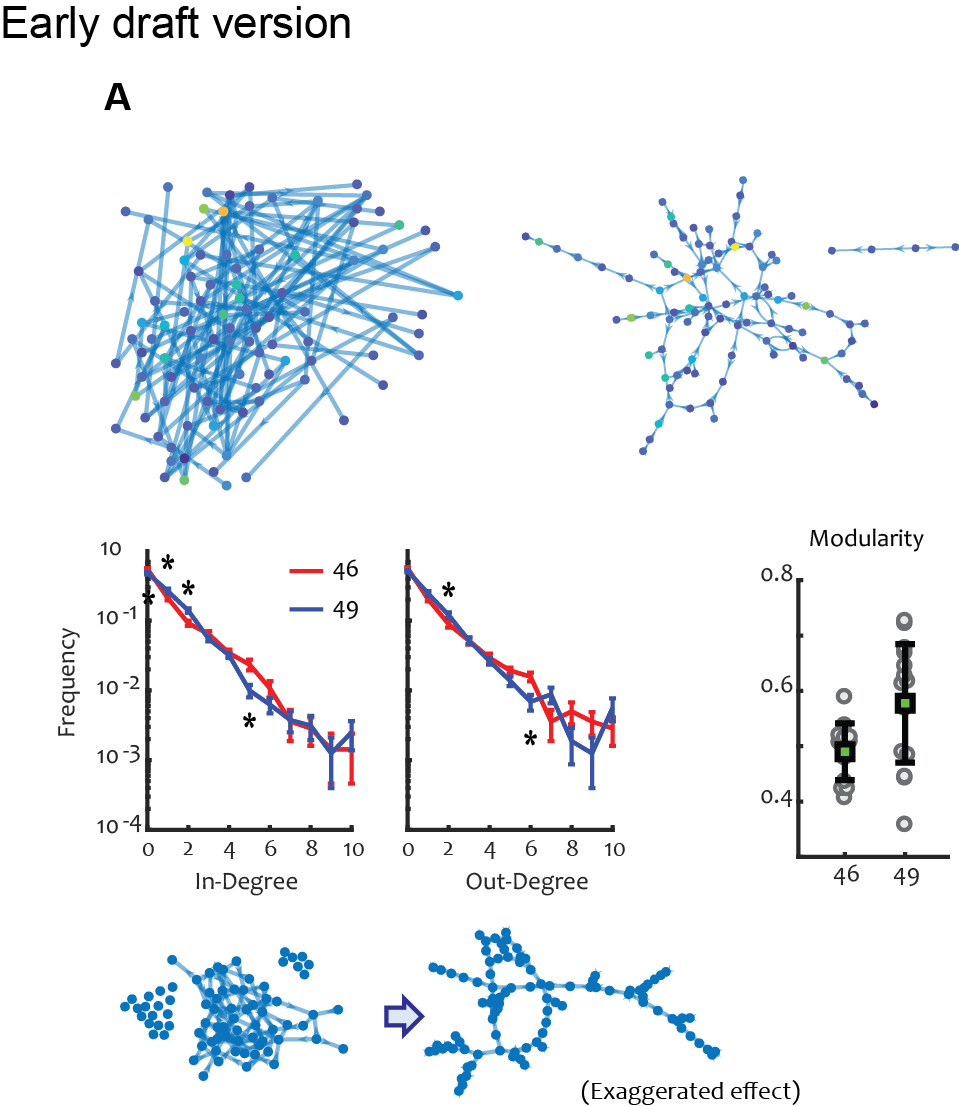
\includegraphics[width=0.5\linewidth]{fig4.png}
\caption{
Spatial variability. \textbf{A}. \textbf{B}. \textbf{C}. \textbf{D}. \textbf{E}. \textbf{F}. }
\end{figure*}

We interpreted transfer entropy values as approximations of weights in an connectivity matrix $\textbf{W}$, with $w_{ji}$ describing the strength of connection from neuron $i$ to neuron $j$ (Fig. 4A). We calculated $\textbf{W}$ and corresponding $p$-values independently on looming, flash, and scrambled stimuli, and used these independent estimations to ensure some level of internal replication within each experiment (see Methods). Of all possible edges, 1.6$\pm$1.4\% were found to be non-zero in all three independent analyses, which was significantly higher than 0.6$\pm$0.09\% expected if edge discoveries were random (paired t-test $p_{tp}=$ 9e-9). Finally, in each experiment, we introduced cut-offs on $w_{ji}$ and $p$-values, to exclude weak noisy edges from the connectivity graph. We automatically adjusted these cut-offs in every experiment, to set the average node degree for each network (the average number of connections per node) as close to 1.0 as possible. It means that in each network, the total number of non-zero edges in the graph was equal to the number of nodes (recorded cells); an approach common for noisy network analysis \citep{stetter2012te}[refs]. With the average total degree set at 1.0, the effective significance thresholds on $p$-values for individual edges were between 0.001 and 0.007 (median 0.004).

The simplest statistical property of a probabilistic networks is its \textbf{degree distribution}: the share of nodes with different number of incoming ($k_{in}$) and outgoing ($k_{out}$) connections. We compared rounded weihgted degree distributions (see Methods) between networks detected in younger and older tadpoles (Fig. 4B), and found that more developed networks contained fewer unconnected cells ($k_{in}$=0, $p_t<$0.03) and fewer cells with high number of connections ($k_{in}$=5, $k_{out}$=6, $p_t$=0.01 in both cases), but more cells with intermediate number of connections ($k_{in}$=2, $p_t$=0.001, and $k_{out}$=2, $p_t$=0.04). When we approximated degree distributions (excluding $k$=0) with a power law (Fig. 4C), the power constant $\gamma$ was smaller in younger (1.48$\pm$0.19) than in older tadpoles (1.82$\pm$0.25, $p_t$=2e-4). The degree distribution became sharper, with a steeper drop between the occurrence rate of weakly connected and highly connected cells. It shows (Fig. 4D) that more developed tectal networks had more linear chains of connected neurons (degree $k$=1) and forks ($k$=2), while younger neurons had more hyperconnected hubs ($k>$5) and unconnected nodes ($k_{in}$=0), as expected for STDP-driven networks \citep{fiete2010chains}.

An unusual feature of our calcium imaging protocol, compared to most calcium imaging techniques, was that the signal-to-noise ratio varied greatly from one cell to another, depending on how far it was from the focal plane, and how much dye it absorbed while partially exposed to chamber solution during staining. As a result, the share of cells with weak signals, that appeared unconnected to the rest of the network due to low pairwise transfer entropy, varied across experiments, and was dependent on extraneous parameters, such as the physical curvature of the preparation. To ensure that poorly resolved cells do not bias our analysis too strongly, we restricted network analysis to the largest weakly connected component of each network. There was no difference in the number of weakly connected components detected in younger and older tadpoles (50$\pm$14 and 50$\pm$26 for stages 45 and 49 respectively, $N$=14 and 16; $p_t$=0.9), but in older animals the largest weakly connected component included a higher share of observed cells (50$\pm$6\% and 64$\pm$12\% respectively; $p_t$=4e-4), matching the changes in degree distributions that we just described.

Synaptic connections in the tectum exhibit robust spike-time dependent plasticity (STDP) \citep{mu2006stdp,pratt2008recurrent}, and a known effect of maturation in networks dominated by STDP is that with time neuronal connections become highly asymmetric. Indeed, if cells $i$ and $j$ are reciprocally connected, every time $j$ spikes after $i$, STDP would increase weight $w_{ij}$ , but diminish weight $w_{ji}$ \citep{abbott1996ltpsequence,fiete2010chains}. We found that in our data, \textbf{the share of bidirectional edges} (with both $w_{ij}$ and $w_{ji}>$0) among all detected edges was smaller (0.3$\pm$0.3\%) than expected for random edge rearrangement in graphs of our size (0.4$\pm$0.1\%, paired $p_t$=0.02), indicating asymmetric information flow in the tectum. Moreover, the share of bidirectional edges decreased in development, from 0.4$\pm$0.3\% in younger animals to 0.2$\pm$0.2\% in older animals ($p_t$=0.03), suggesting that STDP is shaping emerging network topology at these developmental stages.

We then looked at whether connected cells were more likely to be located closer to each other in the tectum. We found that the \textbf{average distance between connected cells} was indeed shorter than the average distance we would get on a randomized graph: 18$\pm$10\% shorter for stage 45, and 17$\pm$8\% shorter for stage 49 tadpoles (individually significant with $p_t<$0.05 for 13/14 and 16/16 experiments respectively). Contrary to our expectations, and in contrast to what is known about visual inputs to the tectum \citep{tao2005refinement}[refs], the intra-tectal connectivity did not become more compact in development ($p_t$=0.7). This may suggest that tectal networks rely on far-reaching recurrent connections to integrate visual information across the visual field \citep{baginskas2009recurrent,liu2016jumbo,jang2016}.

\subsection*{Network properties}

We measured several standard network properties for every connectivity graph reconstructed from tadpole tecta. For each age group, we used two approaches to check whether our network properties were statistically unusual. First, we compared network properties of our graphs to properties of randomly rewired graphs, in which the distribution of edge weights $w_{ji}$, and the number of edges adjacent to each node (node degrees) were kept fixed. This procedure is called degree-preserving rewiring \citep{maslov2002}. Second, we performed a similar comparison, but also randomized node degrees, by reassigning existing edges among all possible edges in a graph (full randomization). In theory, two different modes of randomization allowed us to ascribe non-randomness of observed network parameters to either non-random degree distribution, or non-randomness of mesoscale graph structure \citep{ansmann2012surrogate}. We also compared network statistics between younger and older tadpoles, to see whether network properties changed in development.

The measure of mesoscale connectivity in the graph, named weighted \textbf{network efficiency}, is defined as the average inverse shortest path, for any two nodes in the network \citep{rubinov2010toolbox,latora2001efficiency}. This value is high when, on average, there is a short path between any two randomly chosen nodes, and so signals can be easily propagate within the graph; the value is low when some nodes are located far from each other on a graph (Fig. example). Traditionally, this measure interprets graph edges as pairwise distances between the nodes, with high value edges representing weak connections; for a graph of weights however, high value edges represent strong connections, so network efficiency is calculated on inverse weights $R_{ji} = 1/w_{ji}$ \citep{rubinov2010toolbox}. In our experiments, network efficiency (0.004$\pm$0.002 for stage 46, 0.002$\pm$0.002 for stage 49 tadpoles) was slightly lower than expected for a random network with matching degree distribution ($d$=$-$0.3, paired $p_t$=0.04 and $d$=$-$0.3, paired $p_t$=0.06 for younger and older tadpoles respectively), or a fully randomized network with the same distribution of edge weights ($d$=$-$0.5 and $-$0.05; paired $p_t$=0.02 and 0.01 for younger and older tadpoles respectively). Efficiency did not seem to change in development ($d$=$-$0.8, $p_t$=0.06).

Network \textbf{clustering coefficient} describes the small-scale heterogeneity in the network \citep{fagiolo2007}, and is defined as the relative frequency of two neighboring nodes forming a triangle via a third node that is connected to both of them (Fig. example). The value of clustering coefficient in our networks was small (2.4$\pm$2.5 e-3 for stage 46, 1.5$\pm$1.6 e-3 for stage 49 animals), but was still slightly larger than expected in a rewired network with same degree distribution ($d=$ 0.5 and 0.6, paired $p_t=$ 0.01 and 0.02 for younger and older animals), and similar to what would be expected for a random graph ($d=$ 0.1 and 0.2; paired $p_t=$ 0.4 and 0.3). This suggests that the observed distribution of degrees made the network less clustered than a random network, but the assortative arrangement of nodes countered this effect. There was no change in clustering in development ($d$=$-$0.4, $p_t$=0.3, Fig.).

The network \textbf{modularity} is the most commonly used measure of mesoscale network heterogeneity \citep{leicht2008community,newman2006modularity}. A network with high modularity can be split into a set of sub-networks, with higher density of connections within each sub-network, and weaker connections between sub-networks (Fig. example). In our experiments, the modularity of reconstructed networks did not differ from randomized networks with the same degree distribution ($d=$ 0.2 and 0.3, paired $p_t=$ 0.2 and 0.06, for stages 46 and 49 respectively). Randomized networks with matching degrees, however, were significantly less modular than a matching network ($d$=$-$0.6 and $-$0.4, paired $p_t =$ 3e-7 and 5e-5 respectively). The network modularity also increased in development ($d=$ 1.0, $p_t =$ 0.01), mostly due to changes in edge weights, as this effect did not disappear after random rewiring before comparison (for permutation rewiring, $d=$ 1.2, $p_t=$ 0.003).

The property of \textbf{hierarchical flow} is a derivative measure \citep{mones2012hierarchy} that we based on the distribution of Katz centrality values \citep{katz1953original,fletcher2018katz} (see below) within the network. Intuitively, flow hierarchy is high when connections between nodes largely point in the same direction, as it happens in layers networks, networks with chains of directed edges, or with activity sinks \citep{czegel2015hierarchy}. We hypothesized that a network of dedicated looming detectors may exhibit flow hierarchy, but the data we observed was hard to interpret, as structural non-randomness and the non-randomness of degree distribution affected hierarchical flow coefficients in opposite ways, with two effects cancelling each other. Indeed, observed networks were more hierarchical than randomized networks with matching degrees distribution ($d=$ 1.5 and 1.1, paired $p_t=$ 1e-04 and 1e-03 for younger and older tadpoles respectively), but randomized networks with matching degrees distribution were substantially less hierarchical than fully randomized networks with matching distribution of $w_{ji}$ ($d=-$4.5 and $-$2.6, paired $p_t=$ 4e-8 and 2e-6 respectively). There was no difference in development ($d=-$0.3, $p_t=$ 0.4).

\subsection*{Selectivity Mechanisms}

Even though the architecture of collision-detecting tectal networks is unknown, it is safe to assume that looming-selective neurons integrate streams of information from different parts of the visual field. We therefore hypothesized that these neurons may be non-randomly located within the detected connectivity graph: for example, receive more feed-forward connections, compared to non-selective cells \citep{litwin2014assemblies}. To investigate this question, for each reconstructed network, we calculated correlation coefficients between looming selectivity of each neuron and values that quantified its positioning within the graph, known as measures of \textbf{centrality}.

Looking at the \textbf{number of incoming connections} (weighted in-degree), we found that in stage 46 tadpoles it did not correlate with selectivity ($r=$ 0.08$\pm$0.24, $p_{t1}=$ 0.2; individual $r>$0 in 9/14 experiments), but in stage 49 tadpoles the correlation was significant, even if small ($r=$ 0.07$\pm$0.13, $p_{t1}=$ 0.03; individual $r>$0 in 12/16 experiments), indicating that in older tadpoles selective cells received slightly more incoming connections, compared to non-selective cells.

As a slightly more advanced way to quantify information sinks, we calculated \textbf{Katz centrality} measure for each neuron \citep{katz1953original,fletcher2018katz}. Nodes with high Katz centrality have many paths leading to them, so a spike originating at random within a graph is more likely to eventually excite one of these nodes, compared to a node with a low centrality value. We found that graphs from younger tadpoles showed no correlation between Katz centrality and looming selectivity ($r =$ 0.08$\pm$0.25, $p_{t1} =$ 0.25, individual $r>$0 in 8/14 experiments), but in older tadpoles Katz centrality correlated with selectivity ($r=$ 0.08$\pm$0.13, $p_{t1}=$ 0.03; individual $r>$0 in 12/16 experiments).

As cells with higher Katz centrality tend to be activated more often \citep{fletcher2018katz}, we checked whether cell selectivity for looming stimuli correlated with its \textbf{average activity} during the recording. We found that for both younger and older animals, actively spiking cells tended to have stronger looming selectivity ($r =$ 0.20$\pm$0.24 and 0.14$\pm$0.19 respectively; in both cases $r$ is significantly $>0$, $p_{t1}=$ 0.01 and 0.01). There was no change in this correlation over development ($p_t=$ 0.4).

If looming-selective cells are gathering information from the network, it was also plausible to hypothesize that they would be more likely to be connected to each other, rather than to non-selective cells. To test this, we used the weighted \textbf{assortativity of selectivity} values: a correlation between selectivity scores of every pair of cells connected by an edge, with strength of this edge factored in this calculation as a weight (see Methods). We found that selectivity of connected cells did not correlate in graphs reconstructed from younger tadpoles ($r$=0.05$\pm$0.12, $p_{t1}$=0.14, individual $r>$0 in 9/14 experiments), but correlated in graphs reconstructed from older tadpoles ($r$=0.05$\pm$0.07, $p_{tq}$=0.01; individual $r>$0 in 11/16 experiments). Together, these results suggest that the distribution of selective cells in developed networks became less random, which may indicated a higher role of distributed network calculations in older animals.

We also hypothesized that on average selectivity for looming stimuli may gradually “accumulate” as the signal propagates through the network, and so “downstream” cells on the receiving end of a strong edge within the graph would, on average, be more selective than “upstream” cells. This hypothesis proved to be wrong in both younger and older tadpoles: across all experiments, 52$\pm$7\% of strong edges (top 25\% of $w_{ji}$ values) led from cells with less to more selective cells, which is not different from chance rate ($p_{t1}$=0.1 for analysis across experiments, $n$=30). A weighted average increase in selectivity between two cells connected by an edge was 0.02$\pm$0.07 ($p_{t1}$=0.2, $n$=30), and there was no change in this value in development ($p_t$=0.2, $n$=14, 16).

\subsection*{Developmental Model}

\begin{figure*}[t!]
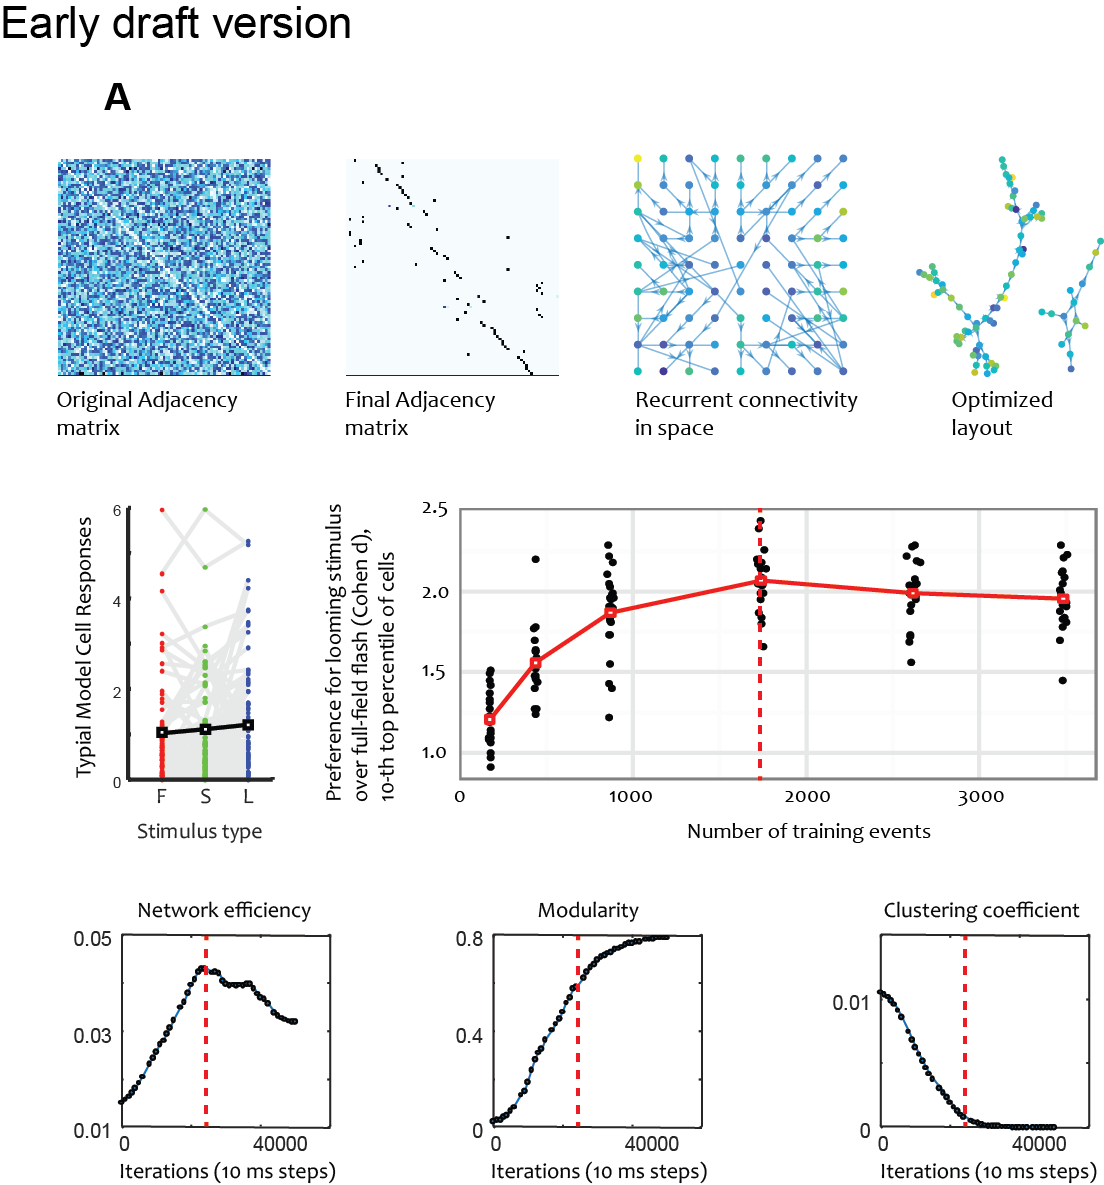
\includegraphics[width=\linewidth]{fig6.png}
\caption{
Spatial variability. \textbf{A}. \textbf{B}. \textbf{C}. \textbf{D}. \textbf{E}. \textbf{F}. }
\end{figure*}

As the networks we studied are complex and noisy, it was hard to provide a clear mechanistic interpretation of our results, especially as in some cases when we used alternative ways to quantify the same intuition, we found the evidence conflicting. For example, for statistical network properties, the effects of non-random degree distribution and mesoscale graph structure often affected network properties in opposite directions (Fig), leading to small total effects. Similarly, when we tried to quantify how “integrative” was the position of each cell within the connectivity graph, only some of these measurements correlated with cell selectivity for looming stimuli, and it was not clear which of these measurements are objectively “better”, in terms of reflecting the true properties of the network.

To compensate for these limitations, and to provide a theoretical counterpoint to our observations, we built a mathematical model of the developing tectum, and ran this model through the same set of measurements that we applied to our experiments. The model consisted of 81 artificial neurons, arranged in a 9 by 9 grid, that were originally all connected to each other (every neuron to every neuron) with random positive (excitatory) synaptic weights (Fig). The model operated in 10 ms increments, and we interpreted the output of each neuron as its instantaneous firing rate. At each time frame we looked at the activity of the network in the previous frame, and summed up the inputs each neuron would receive from each other neuron. We then used a sliding logistic function to translate these synaptic inputs into postsynaptic spiking (see “Methods” for details).

To allow the network develop in time, we introduced three simple developmental rules: spike-time-dependent plasticity (STDP), homeostatic plasticity, and synaptic competition. Our implementation of STDP approximated biological STDP, as observed in the tadpole tectum \citep{zhang1998stdp,mu2006stdp}: if two cells were active in two consecutive 10 ms time frames, and they were connected with a synapse, the weight of this synapse was increased. Conversely, if two cells were active within the same time frame, the weight of a synapse connecting them was decreased, as it means that one cell would try to activate another cell after it already spiked. The homeostatic plasticity adjusted excitability thresholds, trying to keep spiking output of each neuron constant on average \citep{pratt2007intrinsic,turrigiano2011}. The synaptic competition attempted to keep the total strength of synaptic inputs to each neuron, as well as the total strength of outputs from each neuron, close to constant, scaling all synapses of both input and output neurons towards a set target every time there was a change in synaptic efficiency \citep{hamodi2016nmda,cohen2002synreview,munz2014hebbian}.

With these three rules at play, we exposed the model to patterned sensory stimulation, modeling retinotopic inputs from the eye. For the main series of computational experiments, we hypothesized that in biological networks, STDP-driven changes may be amplified by a learning signal \citep{savin2014stdpreward,aswolinskiy2015stdpreward} originating either in dimming receptors in the retina \citep{baranauskas2012}, or mechanosensory systems of the hindbrain \citep{pratt2009multisens,felch2016,truszkowski2017}. Therefore, in the main set of experiments, we only exposed our model to looming stimuli (but see sensitivity analysis below). The network was allowed to develop for 12500 time steps, experienced at least 500 looming stimuli, and we saved its topology at five equally spaced time points during this process, from a naive network, to its final state. We ran independent simulations 50 times, and for each network snapshot we analyzed the properties of the connectivity graph, as well as the responses of each network to “model visual stimuli” that included a looming stimulus, a scrambled stimulus, and a full-field flash. We then analyzed these data in the same way as we did for biological experiments.

\begin{figure*}[t!]
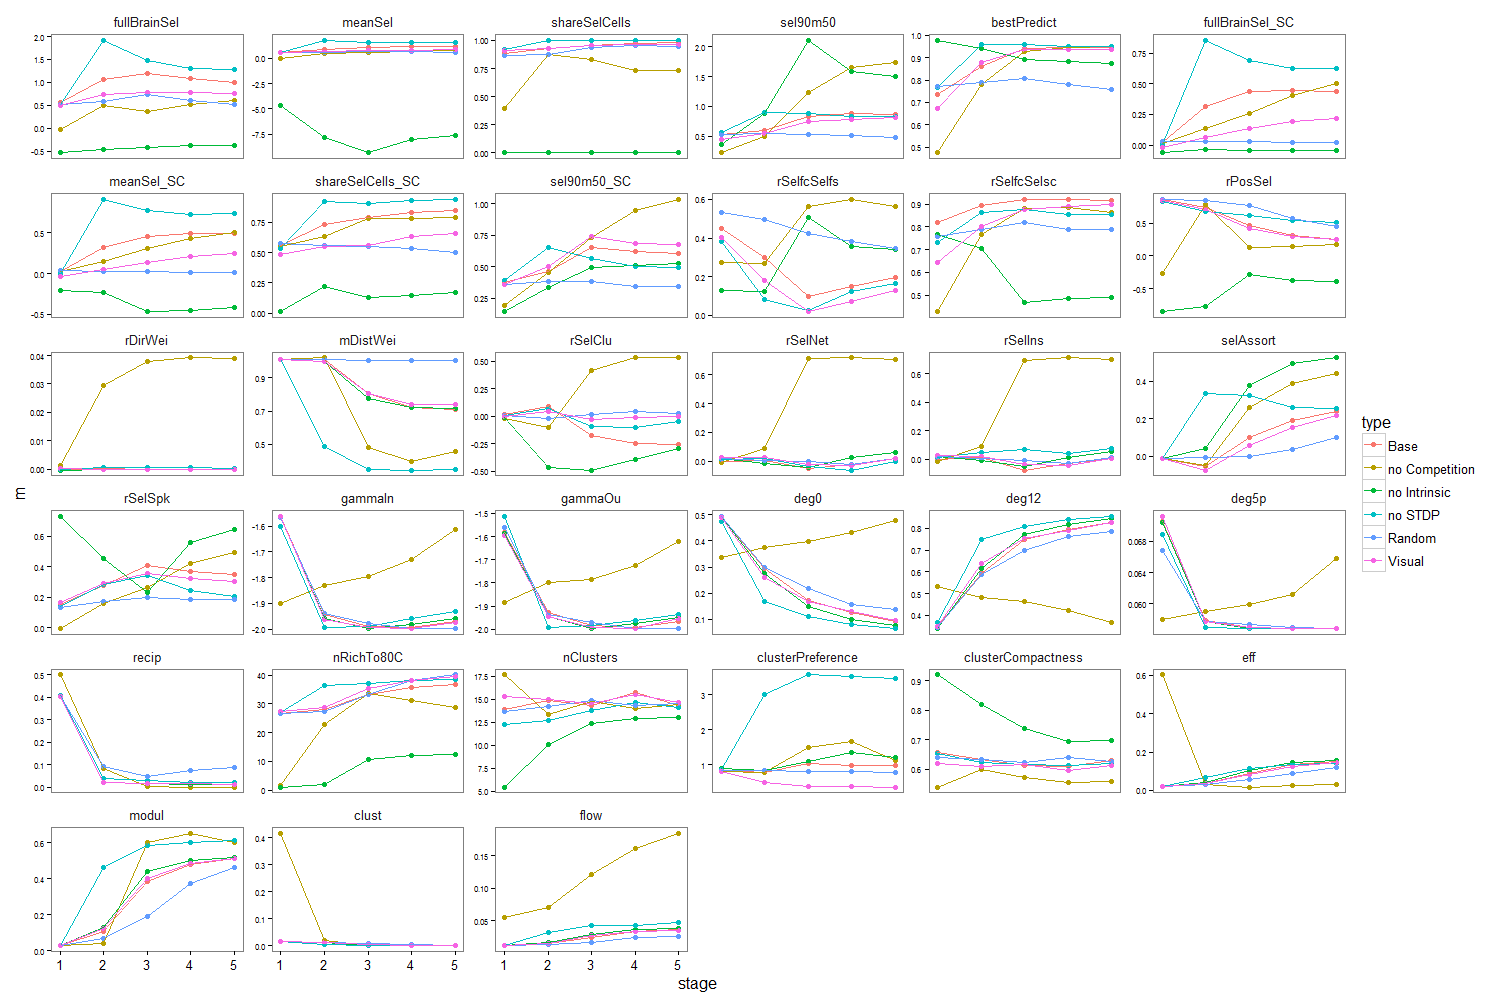
\includegraphics[width=\linewidth]{fig7.png}
\caption{
Model results. \textbf{A}. \textbf{B}. \textbf{C}. \textbf{D}. \textbf{E}. \textbf{F}. }
\end{figure*}

The summary of modeling results is shown in Fig. 7. In development, the network became selective for looming stimuli, both in terms of the total response (by the end of development, responding to looming 99$\pm$9\% stronger than to flash) and mean selectivity (mean Cohen $d$ of responses = 1.09$\pm$0.10). The share of cells selective for looming stimuli also increased, and then saturated at $\sim$98\% level, as did the selectivity of the top 10\% of most selective cells.

To test whether in our model the nature of visual stimuli could be reconstructed from network activation (stimulus encoding), we used a logistic regression on a vector of total cell responses, as it was done for biological data. We then used a different dataset, consisting of equal shares of looming and non-looming stimuli, to assess the accuracy of our model. The prediction power increased in development, and plateaued at the accuracy level of $\sim$95\%. This suggests that a retinotopic STDP-driven network can achieve highly reliable looming detection if it is equipped with an output layer, potentially representing motor neurons in the hindbrain, and the weights of connections to the output layer are set correctly, e.g. via reinforcement learning.

Unlike in biological experiments, the model was selective for looming stimuli over scrambled stimuli at the full network level, and by the end of the training period, responses to looming stimulus were 43$\pm$7\% stronger than to scrambled. Mean selectivity of individual cells, defined as a Cohen $d$ for responses to looming compared to scramble, was 0.48$\pm$0.07, and 84\% of cells were selective for looming stimuli, which is also different from what we observed in biological experiments. The selectivity for looming over flash correlated with selectivity for scrambled stimuli over flash on a cell by cell basis ($r$= 0.17$\pm$0.10). A subset of highly selective cells did not emerge in the model, as the difference between 90th and 50th percentiles of selectivity were rather low ($\sim$ 0.9 ; Fig XXX).

The positioning of selective cells within the network was different in model, compared to biological experiments. While in tadpoles, selective cells tended to be located in the middle of the retinotopic field, in the model they tended to be located on the periphery, and selectivity for looming stimuli positively correlated with the distance from the network center. Similar to tadpoles, however, this correlation disappeared in development (from $r\sim$ 0.75 in a naive network, to $r\sim$0.25 in a trained network). Despite the fact that the edges of looming stimuli generally traveled from the center of the retinotopic field to the periphery, there was no correlation between the weight of a cell-to-cell connection and its being facing outward from the network center ($r$=8e-5), which means that connections were equally likely to face outward and inward. Similarly to biological networks, selective cells tended to be closer to each other (29$\pm$3\% closer) than expected by chance, yet unlike what we observed in biological networks, this locality of connections was refined in developments.

We then looked at topological and functional correlates of looming selectivity in model networks. Selective cells tended to be more spiky ($r$=0.34$\pm$0.12), with very mild increase in development. They tended not to be a part of a cluster (final correlation with local clustering coefficient $r$=$-$0.26$\pm$0.12). Unlike in biological networks, in the model selective sells were not special in terms of their Katz centrality ($r$=0.02$\pm$0.13), and they did not tend to receive an unusual number of incoming connections ($r=$0.00$\pm$0.12). Selective cells tended to be connected to each other (weighted assortativity of 0.24$\pm$0.07), and on average selectivity did not increase over edges ($r$=0.00$\pm$0.14). In naive networks $\sim$85\% of strong edges (top 50\% of edge weights) tended to lead from less selective sells to more selective ones, but in developed networks this share was reduced to chance value (51$\pm$0.03).

The variability of responses to looming stimuli over time, quantified as the number of principal components required to describe 80\% of response variability, mildly increased in development, from 28$\pm$1 to 37$\pm$1. The number of ensembles detected in the network did not change in development, and stayed around 8 to 8.5$\pm$0.5, but the share of variance in network responses explained by the involvement of different ensembles, increased from $\sim$35\% for a naive network, to $\sim$50\% by the end of learning. As in biological results, cells that formed an ensemble were about 10\% closer to each other than random cells in the network, and, in developed networks, were 2.2$\pm$0.5 times more likely to be connected to each other.

The distribution of degrees in the model was similar to that in biological experiments: the share of weakly connected cells (weighted in-degree $<$ 0.5) plummeted from $\sim$50\% in naive networks to 9$\pm$2\% by the end of training. On the contrary, the share of cells with degrees of 1 and 2 increased from $\sim$40\% to 83$\pm$2\%. With this changes, the power constant for the degree distribution changed from $\gamma \sim -$1.5 to $-$1.96$\pm$0.03 for both in- and out-degrees, which also qualitatively matched changes in biological experiments.

Finally, we observed that most network measures changed with network development (Fig): efficiency and modularity increased, while clustering decreased. In all three cases, the changes were mainly due to changes in weight and degree distribution, as they persisted if calculated on networks randomized with degree-preserving rewiring (Fig). The hierarchical flow increased mildly in development, and this was entirely due to structured changes in network topology, as the effect was not present in rewired graphs. A robust increase in modularity may seem to be in contradiction with a stable number of ensembles detected in the network, as network modules are expected to form activity ensembles \citep{triplett2018emergence}. We assume that the reason for this difference was that both in biological and computational experiments, we tried to identify ensembles in highly structured responses, and not in long recordings of spontaneous activity.

To better assess whether the predictions of the model were confirmed in experiments, we formulated a list of “atomic”, elementary statements about each of the measures were analyzed, looking at whether they changed in development, whether they increased or decreased, and whether they differed from similar measures in a randomized network (Table 1, first two columns). Overall, the model and the experiments were similar in flash-looming selectivity, but did not match in terms of scrambled-looming selectivity. The interplay between cell position and connectivity was also similar, except for the spatial distribution of looming-selective cells within the retinotopic map, which was peripheral in the model, but central in tadpoles. Changes in degree distributions were well matched, but except for modularity, other network measures did not match. When correlations between different measures of node centrality and cell selectivity were considered, some of them matched, but many did not.

%\newgeometry{left=1in} % This page will have smaller margins
\begin{table}
    % Help for tables:
% https://en.wikibooks.org/wiki/LaTeX/Tables

\newcolumntype{L}{>{$}l<{$}} % math-mode version of "l" column type
\begin{tabular}{lLLLLLLL}
\textbf{Observation} & 
\multicolumn{1}{|l}{} & 
\multicolumn{6}{|c}{\textbf{Model}}\\
\cline{3-8} &
\multicolumn{1}{|l}{\begin{turn}{90}\textbf{Imaging}\end{turn}} & 
\multicolumn{1}{|l}{
  \begin{turn}{90}Base\end{turn}
} & 
%\text{-STDP} & 
\begin{turn}{90}\text{No STDP}\end{turn} &
%\begin{tabular}{l}No\\Syn.\end{tabular} & 
\begin{turn}{90}\text{No Syn. Comp. }\end{turn} &
%\begin{tabular}{l}No\\Intrins.\end{tabular} & 
\begin{turn}{90}\text{No Instrinsic}\end{turn} &
%\text{Visual} & 
\begin{turn}{90}\text{Visual}\end{turn} &
%\text{Noise} 
\begin{turn}{90}\text{Noise}\end{turn}
\\
\hline
Brain FL selectivity & \checkmark & \checkmark & \checkmark & \checkmark & \times & \checkmark & \checkmark \\
Brain selectivity, change & =	& \land	\lor	& 	\land \lor	& \land & = & \land & =\\
Av. FL selectivity & \text{0.6} & \text{0.8} & \text{1.0} & \text{0.6} & -\text{7.0} & \text{0.8} & \text{0.5} \\
Av. FL selectivity, change & = & \land & \land \lor & \land & \lor \land & \land & = \\
\% FL select. cells & \text{80\%} & \text{98\%} & \text{95\%} & \text{75\%} & \text{0\%} & \text{95\%} & \text{95\%}\\
\% FL select. cells, change & = & \land & \land & \land \lor & = & \land & \land\\
\hline
Brain SL selectivity & \times & \times & \times & \times & \times & \times & \times  \\
Av. SL selectivity & -\text{0.1} & \text{0.5} & \text{0.7} & \text{0.5} & -\text{0.5} & \text{0.2} & \text{0}\\
Av. SL selectivity, change & = & \land & \land \lor & \land & \lor & \land & = \\
\% SL select. cells & \text{50\%} & \text{80\%} & \text{90\%} & \text{70\%} & \text{20\%} & \text{70\%} & \text{50\%} \\
\% SL select. cells, change & = & \land & \land & \land & \land \lor & \land & \lor \\
%SL skew, change & = & \land & \land \lor & \land & - & \land \lor & -\\
cor(FS, FL) & \checkmark & \checkmark & \checkmark & \checkmark & \checkmark & \times & \checkmark \\
cor(SL, FL) & \times & \checkmark & \checkmark & \checkmark & \checkmark & \checkmark & \checkmark\\
Stimulus encoding, change & = & \land & \land & \land & \lor & \land & \land \lor \\
PCA, N components & = & \land & \land & \land \lor & \land & \land & \land\\
\hline
\multicolumn{8}{l}{\textbf{Ensembles:}}\\
N Ensembles, change & = & = & = & \land \lor & \land & = & = \\
Spatial locality & \checkmark & \checkmark & \checkmark & \checkmark & \checkmark & \checkmark & \checkmark\\
Preferential connections  & \checkmark & \checkmark & \checkmark & \checkmark & \checkmark & \times & \times \\
\hline
\multicolumn{8}{l}{\textbf{Connected cells:}}\\
Are spatially close & \checkmark & \checkmark & \checkmark & \checkmark & \checkmark & \checkmark & \times \\
%Get closer in development& \times & \times & \times & \times & \times & \times & \times \\
%Edges point to periphery & = & = & = & \checkmark & = & = & =\\
\% two-way edges, change & \lor & \lor & \lor & \lor & \lor & \lor & \lor \\
%Edges increase selectivity & \times & \times & \times & \checkmark & \times & \times & \times \\
\hline
\multicolumn{8}{l}{\textbf{Network properties:}}\\
%Degree $k=0$, change & \lor & \lor & \lor & \land & \lor & \lor & \lor \\
%Degree $k=1-2$, change & \land & \land & \land & \lor & \land & \land & \land \\
%Degree $k\geqslant 5$, change & \lor & \lor & \lor & \land & \lor & \lor & \lor \\
Degree power ($\gamma$), change & \land & \land & \land & \lor & \land & \land & \land \\
Efficiency, change & = & \land & \land & = & \land & \land & \land \\
Clustering, change & = & \lor & \lor & \lor & \lor & \lor & \lor \\
Modularity, change & \land & \land & \land & \land & \land & \land & \land \\
Hierarchy, change & = & \land & \land & \land & \land & \land & =\\
\hline
\multicolumn{8}{l}{\textbf{Properites of selective cells:}}\\
Center / Periphery location & \text{C} & \text{P} & \text{P} & \text{P} & \times & \text{P} & \text{P}\\
Spatial grouping, change & \lor & \lor & \lor & \lor & \land & \lor & \lor \\
High in-degree $k_{in}$ & \checkmark & \times & \times & \checkmark & \times & \times & \times\\
High Katz rank & \checkmark & \times & \times & \checkmark & \times & \times & \times\\
High activity & \checkmark & \checkmark & \checkmark & \checkmark & \checkmark & \checkmark & \times\\
Assortatively connected & \checkmark & \checkmark & \checkmark & \checkmark & \checkmark & \checkmark & \checkmark\\
%Have unusual clustering coeff. & = & \text{low} & = & \text{high} & \text{low} & = & =\\
\end{tabular}
    \caption{A summary of network phenomena observed in biological experiments, in comparison with the base model, and several reduced models. For clarity, we use $\checkmark$ for "yes", $\times$ for "no", $\land$ for "increase", $\lor$ for "decrease", $\land \lor$ for "increase followed by decrease", and $=$ for "no change". FL stands for "Flash-Looming" comparisons; SL - Scrambled-Looming comparisons; corr denotes correlation.}
\end{table}
%\restoregeometry

\subsection*{Sensitivity analysis}

While a comparison with one faithfully constructed model is important, a better approach is to consider a family of models, and see which elements are critical for the replication of biological results, and which are not essential \citep{linderman2017constrain,pauli2018repro}. For example, in our model, how important was to assume that the plasticity happened in response to a learning signal during actual collisions? Would  looming selectivity develop if instead of unsuccessful looming avoidance we use general visual stimuli? Is structured sensory flow even necessary \citep{triplett2018emergence}? To answer these questions, we repeated our analysis several times, excluding different parts of the model one by one. We first let the model develop while exposed to randomized translational stimuli instead of looming stimuli. In a different set of computational experiments, exposed the model to random visual noise. Then we returned to looming stimuli, but either removed explicit synaptic competition, by replacing it with synapse weight decay; or greatly decreased the amount of intrinsic plasticity present in the system; or replaced STDP with simple symmetrical Hebbian plasticity. The results of these 5 sensitivity experiments are presented in Figure and Table 3, together with curves for the original "full" model.

We found that training specifically on looming stimuli was not critical for the model, but training on structured stimuli (as opposed to noise) was. When looming stimuli were replaced by randomized translational and receding stimuli, almost all network variables still developed similarly to the main series of experiments. Selectivity to looming stimuli, both compared to flash and to scramble, also developed similarly, but reached 20-50\% lower selectivity values (Fig. X-X). In contrast, when patterned stimuli were replaced with uncorrelated noise, selectivity did not improve with time, and while the network still changed its efficiency, modularity, and degree distribution, it did not acquire hierarchical structure, and positioning of selective cells within the graph remained random.

Disruption of different developmental rules led to very different changes in network development (Table XX, Fig. XXX). When STDP was replaced by simple Hebbian plasticity, looming selectivity was similar or better than with STDP, and the network generally developed similarly, except that modularity was higher (Fig X), neuronal ensembles were more strongly interconnected (Fig X), and reciprocal connections between pairs of neurons remained probable (Fig X). This is consistent with the idea that, unlike STDP, Hebbian plasticity does not eliminate tight clusters of strongly interconnected neurons \citep{fiete2010chains}. When synaptic competition was replaced with synaptic strength decay, the degree distribution was very different (got flatter rather than sharper); selectivity for looming stimuli was disrupted; the pattern of interactions between cell selectivity and cell centrality became very much unlike waht was observed in the base series of experiments, and the network became strongly hierarchical. The main reason for these differences appears to be that without synaptic competition, chains of connected neurons may lead to "dead-ends" within the graph, while with competition the total output of each neuron remains approximately constant, which leads to the development of cycles. Finally, when intrinsic plasticity was weakened, the network did not acquire sensitivity to looming stimuli, and had simpler response structure (both in terms of PCA results, and ensemble analysis; Fig X), but retained most of changes in network topology. This suggests that intrinsic plasticity is critical for learning, as without it the network was primarily driven by spontaneous activity, which structured it incorrectly.

\section*{Discussion}

In this study, we hypothesized that a developing network governed by spike-time-dependent plasticity, synaptic competition, and stimulated by patterned visual inputs, would 1) spontaneously develop a non-random network structure, and 2) acquire selectivity for looming stimuli. We also hypothesized that these effects would be robust enough to be replicated in biological experiments. The support for our hypothesis is mixed. The model did develop selectivity for looming stimuli (in terms of both average preference, and distributed stimulus encoding), and this improvement in selectivity was resilient to changes in developmental rules. Yet these seemingly trivial results were not verified in biological experiments, as we observed no improvement in looming detection in development, as neither average selectivity, stimulus encoding, nor cell specialization differed between younger and older tadpoles. This was particularly surprising in view of a known improvement in collision detection with tadpole age \citep{dong2009}.

The model also developed a non-random structure, with several key network properties (efficiency, modularity, clustering, and hierarchy) becoming significantly different from matching values in a randomized network. Most of these properties also changed with model development, yet except for changes in degree distribution and modularity, we did not detect similar network differences between younger and older tadpoles. This may suggest that while neurons in stage 46 and 49 tadpoles have different synaptic and intrinsic properties \citep{ciarleglio2015}, and continue to refine retinal inputs to the tectum \citep{tao2005refinement,munz2014hebbian}, the patterns of internal tectal connectivity may be relatively settled by stage 46. In the model, most network measures plateaued, or even slowly reversed in late development, which means that even for a qualitative comparison between the model and the experiment we have to make an important assumption about whether stage 46 tadpoles correspond to a mid-point of development, or whether they fall on the developmental plateau. The absence of improvement in stimulus identity prediction from neuronal activity in older tadpoles, compared to younger ones, suggests that both stages fall on the “plateau”. If true, this would mean that less robust collision avoidance in behaving stage 46 tadpoles \citep{dong2009} is likely to be due to maturation of sensorimotor connections from the tectum to the hindbrain, which we did not assess in this study.

The changes in degree distribution, observed both in the model and in imaging experiments, were largely a consequence of synaptic competition that explicitly promoted connectivity in underconnected neurons, while "punishing" overconnected cells, creating more light-frame, openwork graph structures \citep{fiete2010chains}. The change in modularity observed in our network supports results previously described in networks governed by Hebbian plasticity \citep{triplett2018emergence,damicelli2018topomod}, and different implementations of STDP \citep{stam2010modular,litwin2014assemblies}. We did not observe changes in the number of neuronal ensembles, but we believe that it is only because our experiments were not well suited for ensemble detection, as we worked with strong shared inputs that reliably activated almost every neuron in the network. This is very different from a case of spontaneous activity, where different sub-networks get activated randomly, with activity propagating within modules more readily than between them \citep{avitan2017spontaneous,pietri2017emergence}.

The sensitivity analysis showed that of all modeling assumptions, the presence of patterned visual stimulation was the most important. The model converged to a state suitable for looming detection even if STDP, synaptic competition, or intrinsic plasticity were disrupted, but it failed if sensory inputs were kept random. Moreover, it was not critical for the model to be trained on looming stimuli: it performed almost as well with a mix of oblique looming, receding, and translating stimuli, which means that it is stimulus locality and edge continuity that mattered for the development. This also suggests that proper tectal network organization can emerge from responses to retinal waves alone, provided that they have spatial and temporal statistics similar to that of behaviorally relevant visual stimuli \citep{huberman2008waves}. Note that our model predicts disrupted tectal organization in enucleated or dark-reared animals, which matches experimental research in tadpoles \citep{xu2011}, but contradicts some experiemntal observations from zebrafish \citep{pietri2017emergence}.

At the same time, to arrange a subset of tectal outputs in a reliable looming detector, a developing brain would need access to both “training” looming stimuli, and a learning signal. We assume that in tadpoles, this learning signal may come from both dimming receptors in the retina \citep{baranauskas2012}, and lateral line receptors in the body \citep{truszkowski2017}. These inputs may trigger plasticity in connections from the tectum to the hindbrain reticulospinal neurons, selecting a subset of inputs that are most active immediately before a collision. Moreover, during random encounters with spatial objects, different parts of the retina would be dimmed, and different segments of the lateral line would be activated in each collision, allowing a tadpole to build several overlapping subnetworks, selective for collisions of different geometry, and projecting to different subsets of motor neurons. Therefore, this type of training could lead to the development of spatially nuanced escape responses that use context to optimize avoidance behaviors, as described in both tadpoles \citep{khakhalin2014} and fish \citep{bhattacharyya2017assessment}.

A relatively poor fit between network predictions and biological experiments may be a consequence of low statistical power of this study. With 14 and 16 networks for two developmental stages respectively, we could only hope to detect changes of Cohen $d \approx$ 1.0, assuming $p_t<$ 0.05 threshold and 80\% power. Moreover, based on available imaging studies, we can estimate that at stage 49, one side of a tadpole tectum contains about 10-15 thousand neurons, as the tectum is about 40 cells across [XXX], and packed 6-10 cells deep in its thickest part [XXX], while tapering towards the edges [XXX]. On the other hand, here we reconstructed connectivity within the top layer of 128$\pm$40 cells, in a field of about 12 by 12 neurons, which means that our reconstructions covered only about 1\% of a full tectal network. With a coverage so sparse, our parameter estimations were expected to be noisy, further lowering the power of our tests.

The best way to address these concerns would be to run a set of control experiment, analyzing transfer entropy between pairs of cells known to be either connected or not, to estimate the actual power of graph reconstruction under these conditions. One possible approach could be to combine Ca imaging recordings with paired whole-cell recordings, probing connections by brief depolarization of one cell and recording of synaptic currents in the other. Unfortunately, this type of experiments was beyond our technical ability, so we had to rely on indirect signs of successful network reconstruction. Two most important observations that support our results, are the fact that the share of reciprocal connections decreased in development; and that we observed a consistent non-randomness of almost all network measurements in reconstructed networks. Also, we were assured by the replication of tectal response shapes (compared to \citep{khakhalin2014}, the internal replication of edge detection between stimuli types (see Methods), and observation of retinotopy during responses to looming stimuli. We therefore conclude that selective staining of neurons in a living brain, followed by high-speed ($\sim$100 frames/s) calcium imaging, allows reconstruction of directed local network connectivity.

\section*{Methods}

\subsection*{Statistics and reporting}

Unless stated otherwise, all values are reported as mean $\pm$ standard deviation. For most common tests, the type of a test is indicated by the subscript for its reported p-value: $p_t$ for a two-sample t-test with two tails and unequal variances; $p_{t1}$ for a one-sample two-tail t-test, and $p_r$ for a Pearson correlation test.

Note also that in this paper we consistely describe adjacency matrices as they are used in computational neuroscience, where $w_{ji}$ is a weight of an edge coming from node $i$ to node $j$, which is different from how adjacency matrices are used in graph theory, where $A_{ji}$ would typically mean an edge from node $j$ to node $i$ (and so $W = A^\top$).

\subsection*{Experiments}

Our experiments followed the procedure previously described in \citep{xu2011,truszkowski2017}, with visual stimulation described in \citep{khakhalin2014}. All experimental procedures were performed at Brown University, in accordance with university IACUC protocols. Except noted otherwise, all chemicals were purchased from Sigma. Tadpoles were kept in Steinberg’s solution, on a 12/12 light cycle, at 18$^\circ$ C for 10-20 days, until they reached Nieuwkoop-Faber developmental stages 45-46 or 48-49. In each experiment, we anesthetized a tadpole with 0.02\% tricainemethane sulfonate (MS-222) solution for 5 minutes, then paralyzed it by immersion in 20 mM solution of tubacurarine for 5 minutes, and pinned it down to a carved Sylgard block within the recording chamber, filled with artificial cerebro-spinal fluid solution (ACSF: 115 mM NaCl, 4 mM KCl, 5 mM HEPES, 10 uM glycine, 10 mM glucose). The optic tectum was exposed, and ventricular membrane was removed on one side of the tectum. Tadpoles were pinned tilted, at an angle of 10-20$^\circ$, to keep the exposed tectal surface flat for imaging. We then surrounded the tadpole with a small circular enclosure 15 mm in diameter, made of a thicker part of a standard plastic transfer pipette, to achieve higher concentration of Ca-sensitive dye in the solution. We dissolved 50 ug of Oregon Green Bapta 1 solution (OGB1 $\#$06807, Molecular Probes, Waltham, MA) in 30 ul of medium consisting of 4\% F-127 detergent in 96\% DMSO by weight; agitated this solution in a sonicator for 15 minutes, then added 30 ul of ACSF to the vial, and sonicated for 10 minutes more. The solution was then transferred to the chamber, mixed with 4 ml of ACSF to the final concentration of 10 uM, and the chamber was placed in the dark for 1 hour. After staining, the circular enclosure was removed; the preparation was washed with 10 ml of ACSF 3 times; the chamber was filled with 10 ml of fresh ACSF, and transferred under the scope.

This staining protocol with a BAPTA-conjugated dye proved to be uniquely challenging, and had a high failure rate. As staining procedure involved a detergent, and called for high concentrations of dye, the most successful preparations were those that received the highest possible exposure that did not yet kill the cells. A large share of preparations however either fell short of optimal staining, and had a weak fluorescence signal, and low signal-to-noise ratio, or got overexposed, leading to strong fluorescence, but weak responses to stimulation, as neurons grew increasingly unhealthy. The variable amount of uncertainty in edge detection from one experiment to another also complicated our network analysis (see below).

Visual stimulation was provided with a previously described setup \citep{khakhalin2014}, consisting of an LCD screen (Kopin Corporation, Taunton, MA, USA) illuminated by a blue LED (LXHL-LB3C, 490 nm; Lumileds Lighting, USA), with the image projected to an optic multifiber (600 um, Fujikura Ltd, Tokyo, Japan). The other end of the fiber was brought to the left eye of the tadpole, and placed 400 um away from the lens, and on the axis of the eye, to have the image projected to the center of the retina. The stimulation sequence consisted of three stimuli: looming stimulus (in which a circle appeared in the center of the field, its radius growing linearly from 0 to full-field within 1 second), full-field flash, and spatially “scrambled” stimulus. For the scrambled stimulus, we divided the field of view into a grid of 17 by 17 squares and randomly reassigned these squares within the image. The result was a stimulus that was identical to looming stimulus in terms of its total brightness at every time step, and presented fragments of a moving edge locally (within every square in a reshuffling grid), but lacked mesoscale spatial organization. The permutation of squares within the grid was randomized for each experiment, but consistent within all trials within an experiment. The stimuli were delivered every 20 s, in a sequence “looming, flash, scrambled”, usually for the total of 60 or 72 stimuli. The stimuli were generated in Matlab (Mathworks), using Psychtoolbox \citep{kleiner2007psychtoolbox}. Imaging excitation light was turned on 1 s before the onset of the visual stimulus, which was shown not to interfere with visual stimulation \citep{xu2011}, and kept on for 5 s.

The tectum was imaged using a Nikon Eclipse FN1 microscope with a 60x water-immersion objective and an ANDOR 860 EM-CCD camera. NIS-elements software (Nikon) was used to record the activity, with binning of 8x8 pixels per bin, resulting in a 130x130 image covering the field of view of 1130 um. The data was acquired with 10 ms auto-exposure, which led to actual frame rate of 84 frames per second (11.9 ms per frame). For each preparation, we used a focal plane that produced images of as many cells as possible, which usually meant a plane focused “in-between” the topmost and bottom-most cells within the field of view. To keep the signal to noise ratio consistent throughout the experiment despite the ongoing bleaching of the Ca sensor, we started with relatively weak illumination (with neutral density filter ND4 engaged) and no signal amplification by the camera (EM gain of 0). We then increased the EM gain level gradually after every 12 stimuli, to keep the signal level approximately constant. Once EM gain setting reached the value of “7”, we increased illumination strength by disengaging one of the density filters, reduced EM gain back to 0, and repeated the process.

Videos were processed offline; circular regions of interest of equal size (21 bins per region) were manually positioned over neurons with well defined, highly variable Ca responses. The average fluorescence within each region of interest was quantified, and exported to Matlab. We processed fluorescence traces with a non-negative deconvolution algorithm \citep{vogelstein2010oopsi}, and used its output without thresholding, interpreting it as an estimation of both timing and number of possible spikes produced by each cell [refs?]. We chose this approach, as depending on the overlap each cell body had with the focal plane, and the amount of dye sequestered, different neurons had very different signal-to-noise ratios, which complicated the matter of finding a single threshold. This decision also shaped all further steps of analysis, as in our dataset both poorly resolved cells with low spiking activity were represented not by spike traces that were mostly silent, but by traces that approached a maximum entropy, uniform distribution of estimator values. For the purposes of deconvolution, in each recording the reference cell was selected automatically, as the cell with 5th highest amplitude fluorescence response.

In this series of experiments, we did not attempt to match inferred spike trains to the “ground-truth” electrophysiological recording from a reference cell, as overall validity of this calcium imaging protocol was justified previously \citep{xu2011,truszkowski2017}. We also did not perform background subtraction [refs], as most effect of background fluorescence were expected to be cancelled out at later stages of analysis. The main risk of not subtracting the background is that unsubtracted traces may contain a superposition of axonal spiking and synaptic activation in the neuropil. In our experiments, the bulk of neuropil activation was expected to be similar in every trial, as stimuli presented to the tadpole were always the same. Moreover, our video acquisition was by design highly sensitive to fluorescence sources lying within the focal plane, which means that the neuropil signal was both greatly attenuated, and spatially averaged. As deconvolution operation is close to linear, and we did not perform spike thresholding, any shared neuropil signal would be deconvolved, “hidden” in inferred spike-trains, and later cancelled out during trial-reshuffling (see below). Finally, we did not address motion artifacts, as in our preparation they were synchronous in all cells (manifested as parallel displacement of signal sources from fixed ROIs), and therefore only introduced a fixed bias to all TE estimations.

\subsection*{Analysis}

\textbf{Basic analysis} For response amplitudes, we used average reconstructed responses between 250 and 2000 ms into the recording, as this window included visual responses, but excluded artifacts caused by the excitation light. As a measure of stimulus selectivity for each cell, and in some cases for the selectivity of total network response, we used Cohen’s $d$ effect size for the difference between responses to looming and flash, or looming and scrambled stimuli:

\[ d = (m_L-m_F)/ \sqrt{ \big((n_L-1) s^2_L + (n_F-1) s^2_F)/(n_L + n_F - 2)} = \]
\[ =(m_L-m_F)/\sqrt{\big(s^2_L+s^2_F\big)/2} \]

in case of equal sample sizes $n_L=n_F=n$. Here $m_L$ and $m_F$ are mean responses to looming and flash stimuli respectively, and $s_L$ , $s_F$ are standard deviations for both groups.

To find the \textbf{retinotopy center}, we concatenated all responses of every cell to looming stimuli into one long vector, ran a principal component analysis on these vectors, then rotated two first components using promax rotation, and made sure that the 1st component $c^1$ is the one with shorter latency, and that it is positive, flipping the components if necessary. We then ran a non-linear optimization, looking for a pair of coordinates for the “retinotopy center” $(x,y)$ that would maximize the absolute value of correlation between distances of each cell to this center and the prominence of the short-latency component in this cell:

\[ r = \text{cor}\big(\sqrt{(x_i-x)^2+(y_i-y)^2}\ ,\ c^1_i/(c^1_i + c^2_i), \big) \]

For \textbf{response latency} calculations, we looked at each response $y(t)$, and found the position of its maximum $(x_M, y_M)$. We then used the least squares fit with non-linear solved to approximate the segment between the beginning of the response and $x_M$ with a piecewise linear function:

\[ f(x) = \left \{ \begin{array}{cll} 0 & \text{for} & 0 \leqslant x<x_L \\
a (x-x_L) & \text{for} & x_L\leqslant x < x_M \end{array} \right. \]

optimizing for $x_L$ and $a$, where $x_L$ is the response latency, and $a$ is an amplitude-like parameter we did not use for subsequent analysis. This approach worked well for isolated responses with good signal to noise ratio, but got increasingly noisy with weak signals. To quantify the retinotopy, we therefore used the results of factor analysis, and only referred to response latencies for verification.

\textbf{Ensemble analysis}. To find ensembles of cells that tended to be co-active together, we used a modified spectral clustering procedure \citep{ng2002spectral} and the definitinon of spectral modularity \citep{newman2006modularity}, generalized to weighted oriented graphs. First, for each stimulus type, for each cell $i$, and separately for each experimental trial $k$, we unbiased and normalized each activity response $a^k_i(t)$, by subtracting its mean, and dividing the result over standard deviation:

\[ a^k_i(t)' = \big(a^k_i(t)-b^k_i\big)/\sigma^k_i \]

where $b^k_i = \sum_{t=1}^T{a^k_i(t)}$ and $\sigma^k_i = \frac{1}{T-1}\sum_{t=1}^T{(a^k_i(t) - b^k_i))}$ .

Then, for each cell, we calculated the average response across all trials of the same type: 

\[ \overline{a_i}(t) = \frac{1}{n}\sum_{k=1}^n{a^k_i(t)} \]

and subtracted these average responses from each trial, which resulted in a vector of a trial-by-trial deviations from the average response:

\[ a^k_i(t)'' = a^k_i(t)' - \overline{a_i}(t) \]

We then used these vectors of deviations from the mean, concatenated across all trials, to calculate a cross-correlation matrix, to see which cells tended to be unusually active or unusually inactive together:

\[ c_{ij} = \text{corr}\big(a''_i(k,t)\, , \, a''_j(k,t)\big) \]

We calculated adjusted correlations $c_{ij}$ separately for each of three types of stimuli (flash, scramble, and looming), and averaged these three estimations $c_{ij}^s$, to arrive at a, hopefully, less noisy estimation of adjusted cross-correlation. We then removed negative correlations, replacing them with zeroes.

\[ c'_{ij} = \text{max}\big(0 \, , \, \frac{1}{3} \sum_{s}{c_{ij}^s}\big) \]

We then roughly followed the spectral clustering approach by \citep{ng2002spectral}, with some adjustments that seemed appropriate for ensemble detection. We first transformed our correlation matrix $c_{ij}$ into a matrix of pairwise Euclidean distances:

\[ \varphi_{ij} = 2(1-c_{ij}) \]

and then to affinity matrix $\textbf{A}$:

\[ a_{ij} = \text{exp}(-\varphi_{ij}/\sigma) \]

where $\sigma$ is a free parameter that we set at 10000. We then calculated a diagonal degree matrix $\textbf{D}$ such that $d_{ij} = 0$ for $i \neq j$ , and $d_{ii} = \sum_k{a_ik}$ otherwise. We used $\textbf{D}$ to build a Laplacian matrix $L$, such as:

\[ L_{ij} = a_{ij}/\sqrt{d_{ii}\cdot d_{jj}} \]

and found eigenvectors $x_1$ .. $x_n$ of matrix $L$. Then we selected a number of ensembles to find $k$, going through all values from 1 (no ensembles) and up to the number of cells (each cell as a separate ensemble). For each $k$, we found first $k$ largest eigenvectors of $L$, stacked them in columns, and renormalized each row of this matrix to give it unit length:

\[ u_{lm} = \frac{x_{lm}}{\sqrt{\sum_{z=1}^{k}{x_{lz}^2}}} \]

where $x_{lm}$ is an $m$-th element of $l$-th eigenvector of $L$. We then used k-means clustering on rows of $\textbf{U}$ as points in $\mathbb{R}^k$, looking for $k$ clusters. Once rows of $\textbf{U}$ (and so cells in the original data) were assigned to $k$ clusters, we calculated spectral modularity of this partition on the original matrix $w_{ij}$, using a weighted directed modification of classic formula from \citep{newman2006modularity}:

\[ Q_k = \frac{1}{4m}\sum_{ij}{\delta_{ij}\Big(w_{ij}-\frac{d^{out}_i d^{in}_j}{2m}}\Big) \]

Here $d^{out}_i$ and $d^{in}_j$ are weighted out- and in-degrees for nodes $i$ and $j$ respectively: $d^{out}_i = \sum_k{w_{ik}}$ , and $d^{in}_j = \sum_k{w_{kj}}$ ; $m$ is the total number of edges involved: $m = \sum_{ij}{w_{ij}}/2$ , and $\delta_{ij}$ is a signal matrix with $\delta_{ij}=1$ for nodes $i$ and $j$ that belong to the same cluster, and $\delta_{ij} = 0$ otherwise. We then found the number of clusters $K$ that, after spectral clustering, produced highest modularity $Q_K$ across all $Q_k$, and used $K$ as an estimation of the number of ensembles in the network, and corresponding cluster allocation - as the allocation of cells to these ensembles.

\textbf{Network reconstruction}. For network reconstruction, we used a modified Transfer Entropy (TE) calculation, adapted from \citep{stetter2012te,gourevitch2007te}. Mathematically, fast Ca imaging recordings, as used in this study, provides a middle ground between commonly used, slower Ca imaging data and multielectrode recordings. In most Ca imaging recordings, the frame acquisition time (100 ms) is an order of magnitude longer than the transmission time between neurons ( 2 ms), which biases analysis towards co-activation analysis. In our data, the high rate of acquisition (12 ms per frame) was very close to typical cell-to-cell activation transmission time in the tectum, so we restricted our analysis to interactions between the activity of each cell at a frame i and their activity at the next frame i+1, ignoring both longer (multiframe), and same-frame interactions.

For each cell, we took its inferred activity train, and binned it at 3 levels, classifying every frame as either a frame with high, medium, or low activity. For each cell, we used 1/3 and 2/3 quantiles of its inferred activity train values as levels thresholds, so that all three types of frames were equally frequent, as this optimized the entropy of representation, while retaining low binning count. Then for each pair of neurons $i$ and $j$ we calculated the probability $P(k_j^1,k_j^0,k_i^0)$, which showed the conditional probability of neuron $j$ being in state $k_j^1$ (either 1, 2, or 3) at moment $t$, if this neuron was in a state $k_j^0$ at the previous frame $t-1$, and  input neuron $i$ was in state $k_i^0$ at the same frame $t-1$. From this set of probabilities, we calculated conditional probabilities of $P(k_j^1 \mid k_j^0)$, and finally calculated the total transfer entropy as

\[ T_{ij} = \sum_{lmn=1}^3{P(k_j^1=l,k_j^0=m,k_i^0=n)}\cdot \log\left(\frac{P(k_j^1=l , \mid , k_j^0=m, , k_i^0=n)}{P(k_j^1=l , \mid , k_j^0=m)}\right) \]

In our project, common drive (visual input from the retina) presents a particular problem. If detection of looming stimuli happens mainly through activation of selected synfire chains, the pattern of this activation would be necessarily synchronized with the causal transfer of excitation from one node to another. Because of that, it cannot be eliminated by methods that rely on the comparison of delays \citep{wollstadt2014te}. Instead, we eliminated the effects of common drive by reshuffling our data, and pairing activation history of each cell with activation history of other cells for reshuffled, unmatching trials recorded in response to same stimulus type. For each experiment, we calculated 1000 randomly reshuffled transfer entropy estimations, and then subtracted the average of these reshuffled TE estimations from our TE estimation, arriving at the value of adjusted TE \citep{gourevitch2007te}:

\[ T'_{ij} = T_{ij} - T^\text{shuffled}_{ij} \]

This approach is similar to the idea of analyzing subtle variations in activation from one response to another, as opposed to the analysis of activation traces themselves. As the stimuli we presented were same in every trial, the progression of the common drive over time was shared across all trials. If a connection between cells $i$ and $j$ was suggested by the analysis of reshuffled data, these cells were clearly sequentially driven by a common input, and not by a true causal connection between them.

For each TE estimation, we also calculated a corresponding p-value, to quantify whether the observed TE was significantly different from the set of TE estimations obtained on surrogate data, corresponding to a null hypothesis of no causal connections, and all network activity due to shared drive. With the computational power available, we could only afford to generate 1000 surrogate reshuffled networks for every TE calculation, which made it impossible to use the false discovery rate correction on our data, as it is recommended for large-scale studies of brain connectivity [Vicente 2011; Lindner 2011]. With $\sim$10$^2$ neurons and 10$^4$ connections the smallest possible non-zero p-value of 0.001, corresponding to finding a more extreme TE value in one out of 1000 surrogate experiments, was already larger than the Benjamini-Hochberg threshold of $\frac{k}{m}\alpha=$5e-6. With a permissive threshold of $\alpha$=0.01, each subset of data (recordings of responses to collisions, flashes, and scrambled stimuli), when taken separately, suggested the existence of 2\% to 69\% of all possible directed edges in the graph, depending on the experiment (median of 8\%). The share of edges that were independently discovered in all three types of experiments (median value of 0.1\% of all possible edges) was on average 1.8 times larger than one would expect in case of spurious and independent discovery (signrank $p$=7e-7), suggesting that the three subsets of data, originating from responses to three different stimuli, can be considered replications for the purposes of edge discovery. At the same time, when we tried to restrict our analysis only to edges that were fully replicated in all 3 sets with $\alpha < $0.05, we ended up with the median graph size of only 18 edges (6 edges in the largest connected component). The overwhelming majority (18 out of 19) of datasets with fewer than 10 reconstructed edges were recorded in the early set of experiments, when our dye transfer from DMSO to ACSF was still imperfect. As during data acquisition, we alternated between stage 46 and 49 tadpoles, the set of “weak” experiments was not biased, and consisted of 10 younger, and 9 older tadpoles. We decided to exclude these 19 “weak” experiments, and believe that restricting all analysis to remaining 30 experiments did not bias the study.

To make the edge inference more robust, for 30 experiments included in further analysis, we relaxed our criteria on edge discovery, while still giving preference to edges discovered independently in more than one subset of responses. To do so, we included in our reconstruction only edges with geometric mean of p-values below significance threshold: $\prod{p_k}<\alpha^3$ , where $p_k$ are p-values for each of three subsets of data (responses to flash, crash, and scrambled stimuli). Because of variation in staining quality and focal plane alignment, we could not use a fixed significance threshold $\alpha$ for all experiments, and instead followed an approach common in analysis of noisy networks, setting the average node degree (the ratio of network edges to network nodes, for directed graphs $=E/N$) to an arbitrary reasonable value \citep{stetter2012te}. For this study, we picked a value of 1.0 (number of edges equal to the number of nodes), which lead to 128$\pm$41 edges in each experiment on average (0.9\% of all possible edges); 50$\pm$21 weakly connected components, and 74$\pm$30 nodes in the largest connected component. The comparison of network properties (Fig) did not change qualitatively in a broad range of assumed average degrees (from $\sim$ 0.5 to 1.5), but observed effects became weaker and regressed to random effects outside of this range.

The TE approach did not distinguish between positive and negative influence of one neuron on another, so our reconstructed edges could include a mix of excitatory and inhibitory connections. To estimate the share of putative inhibitory connections, we calculated pairwise correlations between activities of individual neurons, compensating for the effect of shared inputs through trial reshuffling (similar to how it was done for TE), and looked at the sign of these correlations for pairs of neurons with TE$>$0. We found that 3$\pm$7\% of detected connections seemed inhibitory or inactivating, with no difference between developmental stages ($d$=0.55, $p_t$=0.1). According to our current understanding on the tectal architecture, deepest principal tectal neurons are not expected to be inhibitory [REF?], and the share of negative correlations tended to be lower in experiments with better signal-to-noise ratio, suggesting that at least part of observed inactivating connections may be false discoveries.

To analyze degree distributions, we calculated the sum of weights of incoming and outgoing edges, rounded them towards nearest whole number, and calculated frequencies $F_{in}(k)$ and $F_{out}(k)$ for each degree value $k$. We then fit a regression line $-\gamma k + b$ to a cloud of point $[k , log(F(k)) ]$, for in- and out-degrees separately, estimated two power constants $\gamma_{in}$ and $\gamma_{out}$, and averaged them to arrive at one balanced estimation ($\gamma$).

To quantify the share of reciprocal connections for the model data, we multiplied the weight matrix element-wise on itself transposed, and normalized this value by dividing it on the sum of squared weights: $S=\sum_{ji}{w_{ji} w_{ij}} / \sum_{ji}{w_{ji}^2}$ . This value is equal to 1 for symmetric weight matrices, 0 for matrices without reciprocal connections, and smoothly changes between these two values for "intermediate" all-positive matrices.

\textbf{Network analysis}. We reviewed several lists of statistical and topological metrics of weighted undirected graphs [refs], and selected a sufficiently diverse set of measures that described different aspects of graphs, including average connectivity, unevenness of density, and global structure, and did not change too strongly with the inclusion or exclusion of individual weakly connected nodes. This last point is important, as some topological graph properties, such as cycle order or the presence of “small world” properties, can be very sensitive to the inclusion of only a few weak long-ranged connections \citep{papo2016beware}. We strove to choose network topology measures that would not change catastrophically from one experiment to another because of small variations in the level of noise, or a slightly more generous selection of regions of interests during calcium imaging video quantification, which led us to the following list of network metrics:

\textbf{Global network efficiency}. [refs] was calculated using a function from the Brain Connectivity Toolbox \citep{rubinov2010toolbox} on reciprocals for graph weights $R_{ij} = 1/w_{ij}$, and was defined as:

\[ E = \frac{1}{n} \sum_{i \neq j}^n{\frac{d_{ij}}{n-1}} \]

where $d_{ij}$ is the length of the shortest path $P_{ij}$ connecting nodes $i$ and $j$: $d_{ij} = \sum_{kl \in P_{ij}}{R_{kl}}$

\textbf{Clustering coefficient} \citep{fagiolo2007} was calculated using the Brain Connectivity Toolbox, with a function that supported weighted directed graphs:

\[ C = \frac{1}{n} \sum_i{\frac {t_i}{(k^o_i+k^i_i)(k^o_i+k^i_i-1)-2\sum_j{w_{ij}w_{ji}}}} \]

where $k^o_i$ and $k^i_i$ are out- and in-degrees of node $i$ respectively, and $t_i$ is the weighted number of directed triangles that include node $i$:

\[ t_i = \sum_{j \neq i}{\sum_{k \neq i,j}{w^{1/3}_{ij}w^{1/3}_{jk}w^{1/3}_{ki}}} \]

To estimate \textbf{network modularity}, we used a function from the Brain Connectivity Toolbox, which calculated spectral modularity on a weighted directed graph \citep{reichardt2006community,leicht2008community}.

Our definition of \textbf{hierarchical flow} was inspired by \citep{mones2012hierarchy,czegel2015hierarchy}, but based on the modified Katz centrality \citep{katz1953original,fletcher2018katz}. To calculate Katz centrality, we assumed that on average, each node $j$ collected a flow of incoming signals through all edges $w_{ji}$ leading to this node. The activation arriving through edge $j\leftarrow i$ was proportional to the total activation $z_i$ of node $i$, the weight of this edge $w_{ji}$, a normalization coefficient equal to $1/\text{max}(w_{kl})$, and a damping factor of $d$=0.9. Each node also received a small amount of constant activation $(1-d)$=0.1. The total activation of each node was therefore defined as:

\[ z_j = (1-d) + \frac{d}{\text{max}_{k,l}(w_{kl})} \sum_{i \neq j}{a_i w_{ji}} \]

Each node then further redirected this activation to other nodes. This definition is very close to that of pagerank centrality \citep{page1999pagerank}, with a minor difference that the weights are not normalized to the value of total outgoing weights for each node $i$: that is, we work with raw weights of $w_{ji}$ rather than $w_{ji}/\sum_k{w_{ki}}$. It means that a node with many outputs has a strong influence over network activation, nodes with weak outgoing edges act almost as dead-ends. Similar to a standard pagerank algorithm, we found solution the stable solution of this problem iteratively, by initializing the network with equal values of centrality, and then running the equation above 100 times or until convergence. Once the distribution of centralities $z_i$ stabilized, we used the difference between the maximal Katz centrality and mean centrality across all nodes as a measure of hierarchical flow in the network [ref]: $h = \text{max}(z_i) - \text{mean}(z_i)$.

To check whether network values described above were different from values expected on a random graph, we performed a two-stage \textbf{graph randomization}. First, we randomized each graph using a variety degree-preserving reshuffling \citep{maslov2002}. To do so, for a network with $N_E$ edges we picked 3$\cdot N_E$ random pairs of nodes (nodes $i$, $j$, $k$, and $l$) that had strong connections from $i$ to $j$, and from $k$ to $l$, but weak connections from $i$ to $l$, and from $j$ to $k$ (we required $w_{ji}>w_{li}$ and $w_{lk}>w_{jk}$). We also required all four nodes be different ($i \neq j \neq k \neq l$). Then we cross-wired them, thus gradually randomizing network topology:

\[ \left \{ \begin{array}{l}  
w_{ji} \leftarrow w_{li} \\ 
w_{li} \leftarrow w_{ji} \\
w_{lk} \leftarrow w_{jk} \\
w_{jk} \leftarrow w_{lk}
\end{array} \right. \]

This approach to degree-preserving randomization is slightly different from the original formulation by \citep{maslov2002} in two ways. First, we explicitly don’t allow loops (self-edges) by requiring all four nodes be different. Second, we allow nodes $i$ and $k$, as well as $l$ and $j$ to be connected before the rewiring, and just swap corresponding edge weights, which seems to be a necessary adjustment for directed weighted graphs. It also means that, strictly speaking, for a weighted graph, our randomization only preserves out-degrees, but not in-degrees. Because of the requirement that $w_{ji}>w_{li}$ and $w_{lk}>w_{jk}$, for a binary directed graph our algorithm preserves in-degrees strictly, as it becomes identical to version by Maslov, while for nearly-binary graphs (bimodal or sparse), it tends to preserve in-degrees on average.

Then, at the next step, we completely randomized connections by randomly swapping weights of edges $w_{ji}$ and $w_{lk}$, including zero weighs, which disrupted both in- and out-degree distributions, and led to a random Erd\H{o}s graph with the same distribution of edge weights as in the original graph. We then compared original network measures (on the actually observed graph) to those calculated on degree-preserving rewired graphs (averaged across 20-50 rewirings), and to those calculated on fully rewired graphs (averaged across same number of rewirings). This allowed us too differentiate between the effects of graph structure, and non-random degree distribution.

We also tested whether the connectivity and position of selective cells within the graph is in any way peculiar, by calculating Pearson correlations between cell selectivity and several different graph centrality measurements. Here, we used three centrality measures: weighted in-degree (the sum of weights of all connections to the node); Katz centrality; and clustering coefficient.

To study the distribution of cell selectivity within the graph, we used \textbf{weighted assortativity} as a measure of non-random association of selective cells into subnetworks. The formula for a mixing coefficient in a weighted directed network is given in \citep{farine2014weighted}, based on the logic from \citep{newman2003mixing} and \citep{leung2007weighted}. The original formula from \citep{newman2003mixing} for an unweighted undirected graph defines a mixing coefficient as a Pearson correlation coefficient between properties of nodes connected by edges, taken over all edges in the graph:

\[ r=\underset{ij: a_{ij}=1}{\text{corr}}(x_i,x_j) \]

leading to the following expression:

\[ r = \frac{\frac{1}{E} \sum{x_i x_j} - [\frac{1}{E} \sum{\frac{1}{2}(x_i+x_j)}]^2} {\frac{1}{E} \sum{(x_i^2+x_j^2)}-[\frac{1}{E} \sum{\frac{1}{2}(x_i+x_j)}]^2} \]

where sums are taken over all connected edges $ij: a_{ij}=1$, and $E$ is the total number of edges.

For a weighted graph an equivalent measure can be introduced by replacing summation over edges to summation over all possible pairs of nodes $ij$, with weights $w_{ij}$ introduced in each sum. The resulting expression can be rewritten in several different ways \citep{newman2003mixing,leung2007weighted,farine2014weighted,teller2014assortative}, with several alternative bulky expressions ultimately describing a weighted correlation calculated across all connected directed edges $ij$ with edge values $w_{ij}$ used as correlation weights:

\[ r=\text{cor}(x_i \, , \, x_j \, , \, w_{ij}) \]

where weighted correlation $\text{cor}(a,b,w)$ is introduced through weighted covariances: 

\[ \text{cor}(a,b,w) = \frac{\text{cov}(a,b,w)}{\sqrt{\text{cov}(a,a,w) \cdot \text{cov}(b,b,w)}} \]

that in turn are defined as: 

\[ \text{cov}(a,b,w) = \frac{\sum_i{w_i \cdot (a_i-\bar{a})(b_i-\bar{b})}}{\sum_i{w_i}} \]

with $\bar{a}$ and $\bar{b}$ representing weighted mean values: 

\[ \bar{a}=\sum_i{w_i a_i}/\sum_i{w_i} \]

Note that this definition seems to differ slightly from the one used in the Brain Connectivity Toolbox \citep{rubinov2010toolbox}.

\textbf{Unreported analyses}. For the sake of transparency, we report the list of measures that were calculated, but were hard to interpret, and so were not included in the final manuscript: four measures of weighted directed degree assortativity (in-in, in-out, out-in, and out-out); pagerank centrality; Katz centrality on reversed graph $W'$; hierarchical flow for reversed graph; node reach on direct and reversed graphs (unweighted analog of Katz centrality without attenuation); as an alternative measure of cell selectivity, McFadden’s pseudo-$R$ for a logistic fit of stimulus identity to the total response of each cell, as an alternative measure of cell selectivity. We also made several attempts to estimate the prevalence of directed cycles in our networks, but realized that these new measures require excessive  validation.

\subsection*{Developmental Model}

The model consisted of $n$=81 cells, arranged in a 9x9 grid. The model operated in discrete time, and was run for 500 epochs, 25 time steps each, or for $T$ = 12500 time steps total. Each cell was characterized by three values: its current activity $s_i(t)$ that represented its instantaneous firing rate; spiking threshold $h_i(t)$ that slowly changed over time, and a constant $\hat{s_i}$ that described the target spiking rate for each cell. The target spiking rates $\hat{r_i}$ were randomly assigned at the beginning of each simulation, and were distributed normally around 5/$n$ with a standard deviation of 1/$n$, which means that once these target spiking rates were matched, on average, at any time step, 5 out of 81 cells would be spiking. The spiking thresholds $h_i$ were initialized at the beginning of each simulation with a value $h_i(0) = 1/(n \hat{s_i}) + \mathcal{N}(0,0.1)$, where $\mathcal{N}(0,0.1)$ is a random value, normally distributed around 0 with a standard deviation of 0.1.

Cells were connected to each other with “synapses” of different strengths, represented by a weight matrix \textbf{W}, with weight $0 \leqslant w_{ji} \leqslant 1$ leading from cell $i$ to cell $j$. At the beginning of each simulation the weights were assigned random values, uniformly distributed between 0 and 1, except for self-connections (loops, $w_{ii}$) that were set to 0.

At each time step we first calculated the raw activation \textbf{A} of all neurons: $\textbf{A} = \textbf{WS} + \textbf{B}$, where \textbf{W} is the connectivity matrix, \textbf{S} is the vector of instantaneous spiking rates $s_i$ , and \textbf{B} is the sensory input (see below). For one cell, we have:

\[ a_i(t+1) = \sum_j{w_{ij}s_j(t)} + b_i(t) \]

These raw activation values were then adjusted down, by a formula representing global feedback inhibition, which helped to avoid run-away excitation early in development:

\[ a'_i(t+1) = \left \{ \begin{array}{l l} a_i(t+1)
& \text{if } \sum_j{s_j(t)} \leqslant \zeta \\ 
 & \\
a_i(t+1)\Big/ \Big(1 + \big(\sum_j{s_j(t)} - \zeta\big) \cdot \exp(- t/\tau_e)\Big) 
& \text{otherwise.} \end{array} \right. \]

Here $a'_i(t)$ is the final, adjusted value of activation for every cell; $\sum_j{s_j(t)}$ is the total sum of all cell activities at the previous time step; $\zeta$ is a constant that sets the level of total activity at which inhibition “turns on”, and that in our case was set to the size of the grid of cells \mbox{$\zeta=$ 9}. The exponent $\exp(-t/\tau_e)$ serves as an “easing” function that gradually “eases” the network from inhibition-dominated mode of operation to “free” operation, with a time constant $\tau_e=$ 0.056. This “easing” formula was a practical compromise that greatly sped up our computational experiments, as it dampened network activity early on, when network was still close to randomly connected, and so prone to seizure-like activity, but allowed the simulation run on its own later in development.

The activity of each neuron $s_i(t)$ was then calculated from its total activation $a'_i(t)$:

\[ s_i(t) = g_i\big(a'_i(t)\big) \]

using a logistic activation function: 

\[ g_i(a) = 1/\Big(1+\exp\big(c\cdot(h_i(t)-a)\big)\Big) \]

where $c$ is a steepness parameter, set at $c=$ 20, and $h_i(t)$ is the current spiking threshold of cell $i$. At the beginning of each simulation, spiking thresholds $h_i(0)$ were set to random values, uniformly distributed in a narrow band between $1/(n \hat{s_i})$ and $1/(n \hat{s_i}_i)+0.1$ . During the simulation, the thresholds $h_i(t)$ were updated at each time step, to model the effect of \textbf{intrinsic homeostatic plasticity}. For this purpose, for each cell, we kept track of its running average spiking rate $\bar{s_i}(t)$, and updated both average spiking rates and spiking thresholds $h_i(t)$ by the following formulas:

\[ \bar{s_i}(t+1) = (1-\kappa)\bar{s_i}(t) + \kappa s_i(t) \]

\[ h_i(t+1) = h_i(t) - r_h(\hat{s_i} - \bar{s_i}(t)) \]

where $\kappa=$ 0.05 is a constant that controls the rate of averaging, and $r_h=$ 0.1 is the rate at which spiking thresholds $h_i$ were allowed to adjust, to bring the discrepancy between the target spiking rate $\hat{s_i}$ and running average spiking rate $\bar{s_i}(t)$ to zero.

Once spiking of each neuron at the new time step $s_i(t)$ was calculated, we performed the \textbf{spike-time dependent plasticity} (STDP) step, and adjusted synaptic weights $w_{ji}$ linking neurons in the network. The intuition behind STDP in discrete time can be described by the following system, with options 1 and 2 not being mutually exclusive:

\[ w_{ji}(t+1) = \left \{ \begin{array}{lll} w_{ji}(t)+\epsilon, & \text{if } s_i(t)\neq 0 \text{ and } s_j(t+1)\neq 0 \\ w_{ji}(t)-\epsilon, & \text{if } s_i(t)\neq 0 \text{ and } s_j(t)\neq 0 \\ w_{ji}(t) & \text{if } s_i(t)=0\end{array} \right. \]

where $\epsilon$ is a change in synaptic weight. As in our model neuronal activity $s_i(t)$ was continuous, and we wanted the synaptic change to be proportional to the overlap in neuronal activity, the non-exclusive system above can be rewritten as:

\[ w_{ji}(t+1) = w_{ji}(t) + r_w \big(s_i(t)w_{ji}(t)s_j(t+1) - s_i(t)w_{ji}(t)s_j(t)\big) \]

or

\[ w_{ji}(t+1) = w_{ji}(t)\cdot\Big(1+r_w\big(s_j(t+1)-s_j(t)\big)s_i(t)\Big) \]

where $r_w$ is a constant that controls the level of synaptic plasticity; for this model $r_w$ = 0.25 .

Finally, we modeled \textbf{synaptic competition} by introducing a negative feedback, to limit the total sum of all inputs to each neuron, and all output of each neuron. At every time step, we used the weight matrix $\textbf{W}$ to calculate a modified matrix $\textbf{W}^\text{i}$, with sum of \textit{inputs} to each neuron normalized to a certain fixed value $g$ = 1.5, and a modified weight matrix $\textbf{W}^\text{o}$, for which the total sum of \textit{outputs} of each neuron was normalized to the same value: 

\[ w_{ji}^\text{i} = g \cdot w_{ji}/\sum_k{w_{jk}} \]
\[ w_{ji}^\text{o} = g \cdot w_{ji}/\sum_k{w_{ki}} \]

We then “moved” our actual weight matrix in the direction of the average of these two normalized matrices:

\[ w_{ji}(t+1) = 0.4 \cdot w_{ji} + 0.3 \cdot w^\text{i}_{ji} + 0.3 \cdot w^\text{o}_{ji} \]

Networks were activated with \textbf{simulated visual stimuli} that resembled sensory activation a real animal would have experienced when navigating in a bright-lit environment with sparsely placed black spheres. For general visual stimulation (only used in sensitivity experiments), we repeatedly created unique collision events, with randomized original position of a black sphere relative to the tadpole, final distance to the tadpole, and direction of movement through the visual field. We would then move the projection of this virtual sphere across the virtual retina over a course of $\tau=$ 10 time frames.  When training on looming stimuli (main series of computational experiments), we still initiated objects at random points within the visual field, but made sure that they approached the eye on a "collision trajectory", and at some point covered the entirety of the visual field. When training on noise, we generated random noise with $\zeta=$ 9 pixels flicking on at any given time. For looming and "general visual" stimuli, a projection of a sphere on the virtual retina was a solid circle, with its center moving linearly $(x,y) = (x_0,y_0)+(v_x,v_y)\cdot t/\tau$, and circle radius changing as $R(t) = R_0/(d_0 - v_z \cdot t/\tau)$. The virtual retina consisted of 81 pixels, arranged in a 9x9 grid, that generated both "ON" and "OFF" responses without delay or bursting, as an exclusive OR of two consecutive projections $\text{in}(t) = \text{XOR}(\text{img}(t),\text{img}(t-1))$, and had one-to-one projections to nodes in the model network.For testing, we compared responses to flashes, crashes, and scrambled stimuli. "Crashes" were different from looming stimuli in that the change of projection radius with time was linear $R(t) = \zeta/2 \cdot \sqrt{2} \cdot t/\tau$, rather than realistic; this was because we used linearly expending looming stimuli in biological experiments, both in this study, and in earlier studies \citep{khakhalin2014}. "Scrambled" stimuli were identical to "Crashes", but with all 81 pixels randomly reassigned. "Flashes" were modeled as very fast looming stimuli that took exactly 2 frames to fill the entire field of view, and with pixels reshuffled; as our model was deterministic, we had to use this approximation to introduce some variability into responses to flashes, while keeping them as close to instantaneous as possible.

While testing networks trained on different sensory stimuli, we ran into a surprising complication: during training, different stimuli provided different levels of average activation, and so not only differently shaped synaptic connections between different cells, but also, because of intrinsic plasticity, resulted in neurons acquiring different activation thresholds. This difference in excitability however was an artifact of our training method, and did not approximate any real biological phenomena, as in real tadpoles visual stimuli are expected to be relatively sparse, while we fed all stimuli to the network as one intense train with no gaps. We therefore decided to let all spiking thresholds settle down before testing, to a state that was dependent only on synaptic connectivity, and not on recent stimulation history. We let the model develop for 2000 additional time steps, with only homeostatic plasticity rule on, but without STDP or synaptic scaling, while feeding all neurons with Poisson random noise that activated on average $\zeta$ = 9 neurons at each time step. 

The effect of this additional calibration step was so prominent in the model, that we hypothesize that it may be indirectly relevant to the biological tectum as well. To maintain the network of synaptic connections, each ensemble of synfire chains has to be regularly activated, yet the more active it is, the less excitable the neurons become, making it less likely to "win" during competition with other ensembles during stimulus detection. The dynamics of plasticity in the brain would therefore pose a meta-balancing problem \citep{zenke2017temporal}: if intrinsic plasticity is too flexible, the network that detects unusual stimuli, will get spontaneously activated in the absence of these stimuli, producing high false-positive rate, and will quickly habituate to actual stimuli, but will have no trouble maintaining synaptic connections required for stimulus detection \citep{litwin2014assemblies}. If however intrinsic plasticity is too slow, the network may find it easier to maintain “optimal” levels of sensitivity, but may have trouble maintaining synaptic connections between stimulus presentations \citep{triplett2018emergence}, as low sensitivity would mean low rate of spontaneous replay. The potential solution to this problem may involve either transitioning through distinct developmental stages with different levels of intrinsic plasticity (similar to how we did it in the model, and reminiscent of a known spike of excitability in stage 47 tadpoles \citep{hamodi2014,ciarleglio2015}), or distinct maintenance and operation physiological states regulated by modulatory inputs to the network; a description that resembled that for different phases of sleep.

For model \textbf{sensitivity analysis}, we removed or attenuated parts of the model, one part at a time (but not cumulatively). We tried the following combinations:

\textbf{Non-looming stimuli}. In this mode, instead of training the model exclusively on looming stimuli, we let black circles traverse the visual field in random directions, while either staying of constant angular size, increasing in size, or decreasing in size. As a result, this type of stimulation was still spatially patterned, but consisted mostly of translational stimuli, with some oblique looming stimuli and oblique receding stimuli.

\textbf{Random stimulation}. The network was stimulated with random noise. Each “pixels” of the image would fire with the same probability of $1/\zeta$ where $\zeta$=9.

\textbf{No STDP plasticity}. Instead of a described above equation 

\[ w_{ji}(t+1) = w_{ji}(t)\cdot\Big(1+r_w\big(s_j(t+1)-s_j(t)\big)s_i(t)\Big) \]

we used an equation with symmetrical Hebb plasticity, and no negative depression term: 

\[ w_{ji}(t+1) = w_{ji}(t)\cdot\Big(1+r_w\big(s_j(t+1)\big)s_i(t)\Big) \]

\textbf{No synaptic competition}. Instead of sliding renormalization of all inputs and outputs of each neuron, we allowed synaptic weights to decay to zero: $w_{ji}(t+1) = w_{ji}(t)\cdot (1-\beta)$, where $\beta$ = 0.001.

\textbf{Weak homeostatic plasticity}. In the formula for homeostatic plasticity, instead of change coefficient $r_h$=0.1 we used $r_h$=XXX.

\section*{Acknowledgements}

My greatest gratitude is to Carlos Aizenman who encouraged me to try to publish this work as a single author, even though all experiments described here were performed on his equipment, and the materials were paid for by the money from his grant (NSF IOS-1353044). I also thank Heng Xu (Shanghai Jiao Tong University) for his help with first imaging experiments; Joshua Vogelstein (John Hopkins) for his advice on adaptive thresholding; Petko Bogdanov (SUNY Albany), Csilla Szabo (Skidmore College), Gerrit Ansmann (Bonn University), and Jim Belk (St Andrews University) for their help with network science and graph theory, and Sven Anderson (Bard College) for advice on model analysis.

% \section*{Declaration of Interests}

The authors have no conflicts of interest to disclose.

\nolinenumbers
\bibliographystyle{apalike} % For author-year
%\bibliographystyle{unsrtnat} % For Nature-style
\bibliography{refs}

%TC:endignore
\end{document}